
\documentclass[12pt,a4paper]{article}
%%%%%%%%%%%%%%%%%%%%%%%%%%%%%%%%%%%%%%%%%%%%%%%%%%%%%%%%%%%%%%%%%%%%%%%%%%%%%%%%%%%%%%%%%%%%%%%%%%%%%%%%%%%%%%%%%%%%%%%%%%%%%%%%%%%%%%%%%%%%%%%%%%%%%%%%%%%%%%%%%%%%%%%%%%%%%%%%%%%%%%%%%%%%%%%%%%%%%%%%%%%%%%%%%%%%%%%%%%%%%%%%%%%%%%%%%%%%%%%%%%%%%%%%%%%%
\usepackage{amsmath}
\usepackage{amsfonts}
\usepackage{sw2unicode}
\usepackage[UT1]{fontenc}
\usepackage{pmingliu}
\usepackage[left=0.95in,right=0.95in,top=2cm,bottom=2.54cm]{geometry}


\setcounter{MaxMatrixCols}{10}
%TCIDATA{OutputFilter=LATEX.DLL}
%TCIDATA{Version=5.00.0.2606}
%TCIDATA{<META NAME="SaveForMode" CONTENT="1">}
%TCIDATA{BibliographyScheme=Manual}
%TCIDATA{Created=Monday, January 13, 2014 11:43:31}
%TCIDATA{LastRevised=Monday, June 09, 2014 12:27:06}
%TCIDATA{<META NAME="GraphicsSave" CONTENT="32">}
%TCIDATA{<META NAME="DocumentShell" CONTENT="International\Traditional Chinese Article">}
%TCIDATA{CSTFile=Traditional Chinese.cst}

\setmainfont[Mapping=tex-text]{Times New Roman} 
\setsansfont[Mapping=tex-text]{Arial}           
\setmonofont{Courier New}                       
\setCJKmainfont{�L�n������} 
\newtheorem{theorem}{Theorem}
\newtheorem{acknowledgement}[theorem]{Acknowledgement}
\newtheorem{algorithm}[theorem]{Algorithm}
\newtheorem{axiom}[theorem]{Axiom}
\newtheorem{case}[theorem]{Case}
\newtheorem{claim}[theorem]{Claim}
\newtheorem{conclusion}[theorem]{Conclusion}
\newtheorem{condition}[theorem]{Condition}
\newtheorem{conjecture}[theorem]{Conjecture}
\newtheorem{corollary}[theorem]{Corollary}
\newtheorem{criterion}[theorem]{Criterion}
\newtheorem{definition}[theorem]{Definition}
\newtheorem{example}[theorem]{Example}
\newtheorem{exercise}[theorem]{Exercise}
\newtheorem{lemma}[theorem]{Lemma}
\newtheorem{notation}[theorem]{Notation}
\newtheorem{problem}[theorem]{Problem}
\newtheorem{proposition}[theorem]{Proposition}
\newtheorem{remark}[theorem]{Remark}
\newtheorem{solution}[theorem]{Solution}
\newtheorem{summary}[theorem]{Summary}
\newenvironment{proof}[1][Proof]{\noindent\textbf{#1.} }{\ \rule{0.5em}{0.5em}}
% Macros for Scientific Word 4.0 documents saved with the LaTeX filter.
% Copyright (C) 2002 Mackichan Software, Inc.

\typeout{TCILATEX Macros for Scientific Word 5.0 <13 Feb 2003>.}
\typeout{NOTICE:  This macro file is NOT proprietary and may be 
freely copied and distributed.}
%
\makeatletter

%%%%%%%%%%%%%%%%%%%%%
% pdfTeX related.
\ifx\pdfoutput\relax\let\pdfoutput=\undefined\fi
\newcount\msipdfoutput
\ifx\pdfoutput\undefined
\else
 \ifcase\pdfoutput
 \else 
    \msipdfoutput=1
    \ifx\paperwidth\undefined
    \else
      \ifdim\paperheight=0pt\relax
      \else
        \pdfpageheight\paperheight
      \fi
      \ifdim\paperwidth=0pt\relax
      \else
        \pdfpagewidth\paperwidth
      \fi
    \fi
  \fi  
\fi

%%%%%%%%%%%%%%%%%%%%%
% FMTeXButton
% This is used for putting TeXButtons in the 
% frontmatter of a document. Add a line like
% \QTagDef{FMTeXButton}{101}{} to the filter 
% section of the cst being used. Also add a
% new section containing:
%     [f_101]
%     ALIAS=FMTexButton
%     TAG_TYPE=FIELD
%     TAG_LEADIN=TeX Button:
%
% It also works to put \defs in the preamble after 
% the \input tcilatex
\def\FMTeXButton#1{#1}
%
%%%%%%%%%%%%%%%%%%%%%%
% macros for time
\newcount\@hour\newcount\@minute\chardef\@x10\chardef\@xv60
\def\tcitime{
\def\@time{%
  \@minute\time\@hour\@minute\divide\@hour\@xv
  \ifnum\@hour<\@x 0\fi\the\@hour:%
  \multiply\@hour\@xv\advance\@minute-\@hour
  \ifnum\@minute<\@x 0\fi\the\@minute
  }}%

%%%%%%%%%%%%%%%%%%%%%%
% macro for hyperref and msihyperref
%\@ifundefined{hyperref}{\def\hyperref#1#2#3#4{#2\ref{#4}#3}}{}

\def\x@hyperref#1#2#3{%
   % Turn off various catcodes before reading parameter 4
   \catcode`\~ = 12
   \catcode`\$ = 12
   \catcode`\_ = 12
   \catcode`\# = 12
   \catcode`\& = 12
   \y@hyperref{#1}{#2}{#3}%
}

\def\y@hyperref#1#2#3#4{%
   #2\ref{#4}#3
   \catcode`\~ = 13
   \catcode`\$ = 3
   \catcode`\_ = 8
   \catcode`\# = 6
   \catcode`\& = 4
}

\@ifundefined{hyperref}{\let\hyperref\x@hyperref}{}
\@ifundefined{msihyperref}{\let\msihyperref\x@hyperref}{}




% macro for external program call
\@ifundefined{qExtProgCall}{\def\qExtProgCall#1#2#3#4#5#6{\relax}}{}
%%%%%%%%%%%%%%%%%%%%%%
%
% macros for graphics
%
\def\FILENAME#1{#1}%
%
\def\QCTOpt[#1]#2{%
  \def\QCTOptB{#1}
  \def\QCTOptA{#2}
}
\def\QCTNOpt#1{%
  \def\QCTOptA{#1}
  \let\QCTOptB\empty
}
\def\Qct{%
  \@ifnextchar[{%
    \QCTOpt}{\QCTNOpt}
}
\def\QCBOpt[#1]#2{%
  \def\QCBOptB{#1}%
  \def\QCBOptA{#2}%
}
\def\QCBNOpt#1{%
  \def\QCBOptA{#1}%
  \let\QCBOptB\empty
}
\def\Qcb{%
  \@ifnextchar[{%
    \QCBOpt}{\QCBNOpt}%
}
\def\PrepCapArgs{%
  \ifx\QCBOptA\empty
    \ifx\QCTOptA\empty
      {}%
    \else
      \ifx\QCTOptB\empty
        {\QCTOptA}%
      \else
        [\QCTOptB]{\QCTOptA}%
      \fi
    \fi
  \else
    \ifx\QCBOptA\empty
      {}%
    \else
      \ifx\QCBOptB\empty
        {\QCBOptA}%
      \else
        [\QCBOptB]{\QCBOptA}%
      \fi
    \fi
  \fi
}
\newcount\GRAPHICSTYPE
%\GRAPHICSTYPE 0 is for TurboTeX
%\GRAPHICSTYPE 1 is for DVIWindo (PostScript)
%%%(removed)%\GRAPHICSTYPE 2 is for psfig (PostScript)
\GRAPHICSTYPE=\z@
\def\GRAPHICSPS#1{%
 \ifcase\GRAPHICSTYPE%\GRAPHICSTYPE=0
   \special{ps: #1}%
 \or%\GRAPHICSTYPE=1
   \special{language "PS", include "#1"}%
%%%\or%\GRAPHICSTYPE=2
%%%  #1%
 \fi
}%
%
\def\GRAPHICSHP#1{\special{include #1}}%
%
% \graffile{ body }                                  %#1
%          { contentswidth (scalar)  }               %#2
%          { contentsheight (scalar) }               %#3
%          { vertical shift when in-line (scalar) }  %#4

\def\graffile#1#2#3#4{%
%%% \ifnum\GRAPHICSTYPE=\tw@
%%%  %Following if using psfig
%%%  \@ifundefined{psfig}{\input psfig.tex}{}%
%%%  \psfig{file=#1, height=#3, width=#2}%
%%% \else
  %Following for all others
  % JCS - added BOXTHEFRAME, see below
    \bgroup
	   \@inlabelfalse
       \leavevmode
       \@ifundefined{bbl@deactivate}{\def~{\string~}}{\activesoff}%
        \raise -#4 \BOXTHEFRAME{%
           \hbox to #2{\raise #3\hbox to #2{\null #1\hfil}}}%
    \egroup
}%
%
% A box for drafts
\def\draftbox#1#2#3#4{%
 \leavevmode\raise -#4 \hbox{%
  \frame{\rlap{\protect\tiny #1}\hbox to #2%
   {\vrule height#3 width\z@ depth\z@\hfil}%
  }%
 }%
}%
%
\newcount\@msidraft
\@msidraft=\z@
\let\nographics=\@msidraft
\newif\ifwasdraft
\wasdraftfalse

%  \GRAPHIC{ body }                                  %#1
%          { draft name }                            %#2
%          { contentswidth (scalar)  }               %#3
%          { contentsheight (scalar) }               %#4
%          { vertical shift when in-line (scalar) }  %#5
\def\GRAPHIC#1#2#3#4#5{%
   \ifnum\@msidraft=\@ne\draftbox{#2}{#3}{#4}{#5}%
   \else\graffile{#1}{#3}{#4}{#5}%
   \fi
}
%
\def\addtoLaTeXparams#1{%
    \edef\LaTeXparams{\LaTeXparams #1}}%
%
% JCS -  added a switch BoxFrame that can 
% be set by including X in the frame params.
% If set a box is drawn around the frame.

\newif\ifBoxFrame \BoxFramefalse
\newif\ifOverFrame \OverFramefalse
\newif\ifUnderFrame \UnderFramefalse

\def\BOXTHEFRAME#1{%
   \hbox{%
      \ifBoxFrame
         \frame{#1}%
      \else
         {#1}%
      \fi
   }%
}


\def\doFRAMEparams#1{\BoxFramefalse\OverFramefalse\UnderFramefalse\readFRAMEparams#1\end}%
\def\readFRAMEparams#1{%
 \ifx#1\end%
  \let\next=\relax
  \else
  \ifx#1i\dispkind=\z@\fi
  \ifx#1d\dispkind=\@ne\fi
  \ifx#1f\dispkind=\tw@\fi
  \ifx#1t\addtoLaTeXparams{t}\fi
  \ifx#1b\addtoLaTeXparams{b}\fi
  \ifx#1p\addtoLaTeXparams{p}\fi
  \ifx#1h\addtoLaTeXparams{h}\fi
  \ifx#1X\BoxFrametrue\fi
  \ifx#1O\OverFrametrue\fi
  \ifx#1U\UnderFrametrue\fi
  \ifx#1w
    \ifnum\@msidraft=1\wasdrafttrue\else\wasdraftfalse\fi
    \@msidraft=\@ne
  \fi
  \let\next=\readFRAMEparams
  \fi
 \next
 }%
%
%Macro for In-line graphics object
%   \IFRAME{ contentswidth (scalar)  }               %#1
%          { contentsheight (scalar) }               %#2
%          { vertical shift when in-line (scalar) }  %#3
%          { draft name }                            %#4
%          { body }                                  %#5
%          { caption}                                %#6


\def\IFRAME#1#2#3#4#5#6{%
      \bgroup
      \let\QCTOptA\empty
      \let\QCTOptB\empty
      \let\QCBOptA\empty
      \let\QCBOptB\empty
      #6%
      \parindent=0pt
      \leftskip=0pt
      \rightskip=0pt
      \setbox0=\hbox{\QCBOptA}%
      \@tempdima=#1\relax
      \ifOverFrame
          % Do this later
          \typeout{This is not implemented yet}%
          \show\HELP
      \else
         \ifdim\wd0>\@tempdima
            \advance\@tempdima by \@tempdima
            \ifdim\wd0 >\@tempdima
               \setbox1 =\vbox{%
                  \unskip\hbox to \@tempdima{\hfill\GRAPHIC{#5}{#4}{#1}{#2}{#3}\hfill}%
                  \unskip\hbox to \@tempdima{\parbox[b]{\@tempdima}{\QCBOptA}}%
               }%
               \wd1=\@tempdima
            \else
               \textwidth=\wd0
               \setbox1 =\vbox{%
                 \noindent\hbox to \wd0{\hfill\GRAPHIC{#5}{#4}{#1}{#2}{#3}\hfill}\\%
                 \noindent\hbox{\QCBOptA}%
               }%
               \wd1=\wd0
            \fi
         \else
            \ifdim\wd0>0pt
              \hsize=\@tempdima
              \setbox1=\vbox{%
                \unskip\GRAPHIC{#5}{#4}{#1}{#2}{0pt}%
                \break
                \unskip\hbox to \@tempdima{\hfill \QCBOptA\hfill}%
              }%
              \wd1=\@tempdima
           \else
              \hsize=\@tempdima
              \setbox1=\vbox{%
                \unskip\GRAPHIC{#5}{#4}{#1}{#2}{0pt}%
              }%
              \wd1=\@tempdima
           \fi
         \fi
         \@tempdimb=\ht1
         %\advance\@tempdimb by \dp1
         \advance\@tempdimb by -#2
         \advance\@tempdimb by #3
         \leavevmode
         \raise -\@tempdimb \hbox{\box1}%
      \fi
      \egroup%
}%
%
%Macro for Display graphics object
%   \DFRAME{ contentswidth (scalar)  }               %#1
%          { contentsheight (scalar) }               %#2
%          { draft label }                           %#3
%          { name }                                  %#4
%          { caption}                                %#5
\def\DFRAME#1#2#3#4#5{%
  \vspace\topsep
  \hfil\break
  \bgroup
     \leftskip\@flushglue
	 \rightskip\@flushglue
	 \parindent\z@
	 \parfillskip\z@skip
     \let\QCTOptA\empty
     \let\QCTOptB\empty
     \let\QCBOptA\empty
     \let\QCBOptB\empty
	 \vbox\bgroup
        \ifOverFrame 
           #5\QCTOptA\par
        \fi
        \GRAPHIC{#4}{#3}{#1}{#2}{\z@}%
        \ifUnderFrame 
           \break#5\QCBOptA
        \fi
	 \egroup
  \egroup
  \vspace\topsep
  \break
}%
%
%Macro for Floating graphic object
%   \FFRAME{ framedata f|i tbph x F|T }              %#1
%          { contentswidth (scalar)  }               %#2
%          { contentsheight (scalar) }               %#3
%          { caption }                               %#4
%          { label }                                 %#5
%          { draft name }                            %#6
%          { body }                                  %#7
\def\FFRAME#1#2#3#4#5#6#7{%
 %If float.sty loaded and float option is 'h', change to 'H'  (gp) 1998/09/05
  \@ifundefined{floatstyle}
    {%floatstyle undefined (and float.sty not present), no change
     \begin{figure}[#1]%
    }
    {%floatstyle DEFINED
	 \ifx#1h%Only the h parameter, change to H
      \begin{figure}[H]%
	 \else
      \begin{figure}[#1]%
	 \fi
	}
  \let\QCTOptA\empty
  \let\QCTOptB\empty
  \let\QCBOptA\empty
  \let\QCBOptB\empty
  \ifOverFrame
    #4
    \ifx\QCTOptA\empty
    \else
      \ifx\QCTOptB\empty
        \caption{\QCTOptA}%
      \else
        \caption[\QCTOptB]{\QCTOptA}%
      \fi
    \fi
    \ifUnderFrame\else
      \label{#5}%
    \fi
  \else
    \UnderFrametrue%
  \fi
  \begin{center}\GRAPHIC{#7}{#6}{#2}{#3}{\z@}\end{center}%
  \ifUnderFrame
    #4
    \ifx\QCBOptA\empty
      \caption{}%
    \else
      \ifx\QCBOptB\empty
        \caption{\QCBOptA}%
      \else
        \caption[\QCBOptB]{\QCBOptA}%
      \fi
    \fi
    \label{#5}%
  \fi
  \end{figure}%
 }%
%
%
%    \FRAME{ framedata f|i tbph x F|T }              %#1
%          { contentswidth (scalar)  }               %#2
%          { contentsheight (scalar) }               %#3
%          { vertical shift when in-line (scalar) }  %#4
%          { caption }                               %#5
%          { label }                                 %#6
%          { name }                                  %#7
%          { body }                                  %#8
%
%    framedata is a string which can contain the following
%    characters: idftbphxFT
%    Their meaning is as follows:
%             i, d or f : in-line, display, or floating
%             t,b,p,h   : LaTeX floating placement options
%             x         : fit contents box to contents
%             F or T    : Figure or Table. 
%                         Later this can expand
%                         to a more general float class.
%
%
\newcount\dispkind%

\def\makeactives{
  \catcode`\"=\active
  \catcode`\;=\active
  \catcode`\:=\active
  \catcode`\'=\active
  \catcode`\~=\active
}
\bgroup
   \makeactives
   \gdef\activesoff{%
      \def"{\string"}%
      \def;{\string;}%
      \def:{\string:}%
      \def'{\string'}%
      \def~{\string~}%
      %\bbl@deactivate{"}%
      %\bbl@deactivate{;}%
      %\bbl@deactivate{:}%
      %\bbl@deactivate{'}%
    }
\egroup

\def\FRAME#1#2#3#4#5#6#7#8{%
 \bgroup
 \ifnum\@msidraft=\@ne
   \wasdrafttrue
 \else
   \wasdraftfalse%
 \fi
 \def\LaTeXparams{}%
 \dispkind=\z@
 \def\LaTeXparams{}%
 \doFRAMEparams{#1}%
 \ifnum\dispkind=\z@\IFRAME{#2}{#3}{#4}{#7}{#8}{#5}\else
  \ifnum\dispkind=\@ne\DFRAME{#2}{#3}{#7}{#8}{#5}\else
   \ifnum\dispkind=\tw@
    \edef\@tempa{\noexpand\FFRAME{\LaTeXparams}}%
    \@tempa{#2}{#3}{#5}{#6}{#7}{#8}%
    \fi
   \fi
  \fi
  \ifwasdraft\@msidraft=1\else\@msidraft=0\fi{}%
  \egroup
 }%
%
% This macro added to let SW gobble a parameter that
% should not be passed on and expanded. 

\def\TEXUX#1{"texux"}

%
% Macros for text attributes:
%
\def\BF#1{{\bf {#1}}}%
\def\NEG#1{\leavevmode\hbox{\rlap{\thinspace/}{$#1$}}}%
%
%%%%%%%%%%%%%%%%%%%%%%%%%%%%%%%%%%%%%%%%%%%%%%%%%%%%%%%%%%%%%%%%%%%%%%%%
%
%
% macros for user - defined functions
\def\limfunc#1{\mathop{\rm #1}}%
\def\func#1{\mathop{\rm #1}\nolimits}%
% macro for unit names
\def\unit#1{\mathord{\thinspace\rm #1}}%

%
% miscellaneous 
\long\def\QQQ#1#2{%
     \long\expandafter\def\csname#1\endcsname{#2}}%
\@ifundefined{QTP}{\def\QTP#1{}}{}
\@ifundefined{QEXCLUDE}{\def\QEXCLUDE#1{}}{}
\@ifundefined{Qlb}{\def\Qlb#1{#1}}{}
\@ifundefined{Qlt}{\def\Qlt#1{#1}}{}
\def\QWE{}%
\long\def\QQA#1#2{}%
\def\QTR#1#2{{\csname#1\endcsname {#2}}}%
\long\def\TeXButton#1#2{#2}%
\long\def\QSubDoc#1#2{#2}%
\def\EXPAND#1[#2]#3{}%
\def\NOEXPAND#1[#2]#3{}%
\def\PROTECTED{}%
\def\LaTeXparent#1{}%
\def\ChildStyles#1{}%
\def\ChildDefaults#1{}%
\def\QTagDef#1#2#3{}%

% Constructs added with Scientific Notebook
\@ifundefined{correctchoice}{\def\correctchoice{\relax}}{}
\@ifundefined{HTML}{\def\HTML#1{\relax}}{}
\@ifundefined{TCIIcon}{\def\TCIIcon#1#2#3#4{\relax}}{}
\if@compatibility
  \typeout{Not defining UNICODE  U or CustomNote commands for LaTeX 2.09.}
\else
  \providecommand{\UNICODE}[2][]{\protect\rule{.1in}{.1in}}
  \providecommand{\U}[1]{\protect\rule{.1in}{.1in}}
  \providecommand{\CustomNote}[3][]{\marginpar{#3}}
\fi

\@ifundefined{lambdabar}{
      \def\lambdabar{\errmessage{You have used the lambdabar symbol. 
                      This is available for typesetting only in RevTeX styles.}}
   }{}

%
% Macros for style editor docs
\@ifundefined{StyleEditBeginDoc}{\def\StyleEditBeginDoc{\relax}}{}
%
% Macros for footnotes
\def\QQfnmark#1{\footnotemark}
\def\QQfntext#1#2{\addtocounter{footnote}{#1}\footnotetext{#2}}
%
% Macros for indexing.
%
\@ifundefined{TCIMAKEINDEX}{}{\makeindex}%
%
% Attempts to avoid problems with other styles
\@ifundefined{abstract}{%
 \def\abstract{%
  \if@twocolumn
   \section*{Abstract (Not appropriate in this style!)}%
   \else \small 
   \begin{center}{\bf Abstract\vspace{-.5em}\vspace{\z@}}\end{center}%
   \quotation 
   \fi
  }%
 }{%
 }%
\@ifundefined{endabstract}{\def\endabstract
  {\if@twocolumn\else\endquotation\fi}}{}%
\@ifundefined{maketitle}{\def\maketitle#1{}}{}%
\@ifundefined{affiliation}{\def\affiliation#1{}}{}%
\@ifundefined{proof}{\def\proof{\noindent{\bfseries Proof. }}}{}%
\@ifundefined{endproof}{\def\endproof{\mbox{\ \rule{.1in}{.1in}}}}{}%
\@ifundefined{newfield}{\def\newfield#1#2{}}{}%
\@ifundefined{chapter}{\def\chapter#1{\par(Chapter head:)#1\par }%
 \newcount\c@chapter}{}%
\@ifundefined{part}{\def\part#1{\par(Part head:)#1\par }}{}%
\@ifundefined{section}{\def\section#1{\par(Section head:)#1\par }}{}%
\@ifundefined{subsection}{\def\subsection#1%
 {\par(Subsection head:)#1\par }}{}%
\@ifundefined{subsubsection}{\def\subsubsection#1%
 {\par(Subsubsection head:)#1\par }}{}%
\@ifundefined{paragraph}{\def\paragraph#1%
 {\par(Subsubsubsection head:)#1\par }}{}%
\@ifundefined{subparagraph}{\def\subparagraph#1%
 {\par(Subsubsubsubsection head:)#1\par }}{}%
%%%%%%%%%%%%%%%%%%%%%%%%%%%%%%%%%%%%%%%%%%%%%%%%%%%%%%%%%%%%%%%%%%%%%%%%
% These symbols are not recognized by LaTeX
\@ifundefined{therefore}{\def\therefore{}}{}%
\@ifundefined{backepsilon}{\def\backepsilon{}}{}%
\@ifundefined{yen}{\def\yen{\hbox{\rm\rlap=Y}}}{}%
\@ifundefined{registered}{%
   \def\registered{\relax\ifmmode{}\r@gistered
                    \else$\m@th\r@gistered$\fi}%
 \def\r@gistered{^{\ooalign
  {\hfil\raise.07ex\hbox{$\scriptstyle\rm\text{R}$}\hfil\crcr
  \mathhexbox20D}}}}{}%
\@ifundefined{Eth}{\def\Eth{}}{}%
\@ifundefined{eth}{\def\eth{}}{}%
\@ifundefined{Thorn}{\def\Thorn{}}{}%
\@ifundefined{thorn}{\def\thorn{}}{}%
% A macro to allow any symbol that requires math to appear in text
\def\TEXTsymbol#1{\mbox{$#1$}}%
\@ifundefined{degree}{\def\degree{{}^{\circ}}}{}%
%
% macros for T3TeX files
\newdimen\theight
\@ifundefined{Column}{\def\Column{%
 \vadjust{\setbox\z@=\hbox{\scriptsize\quad\quad tcol}%
  \theight=\ht\z@\advance\theight by \dp\z@\advance\theight by \lineskip
  \kern -\theight \vbox to \theight{%
   \rightline{\rlap{\box\z@}}%
   \vss
   }%
  }%
 }}{}%
%
\@ifundefined{qed}{\def\qed{%
 \ifhmode\unskip\nobreak\fi\ifmmode\ifinner\else\hskip5\p@\fi\fi
 \hbox{\hskip5\p@\vrule width4\p@ height6\p@ depth1.5\p@\hskip\p@}%
 }}{}%
%
\@ifundefined{cents}{\def\cents{\hbox{\rm\rlap c/}}}{}%
\@ifundefined{tciLaplace}{\def\tciLaplace{\ensuremath{\mathcal{L}}}}{}%
\@ifundefined{tciFourier}{\def\tciFourier{\ensuremath{\mathcal{F}}}}{}%
\@ifundefined{textcurrency}{\def\textcurrency{\hbox{\rm\rlap xo}}}{}%
\@ifundefined{texteuro}{\def\texteuro{\hbox{\rm\rlap C=}}}{}%
\@ifundefined{euro}{\def\euro{\hbox{\rm\rlap C=}}}{}%
\@ifundefined{textfranc}{\def\textfranc{\hbox{\rm\rlap-F}}}{}%
\@ifundefined{textlira}{\def\textlira{\hbox{\rm\rlap L=}}}{}%
\@ifundefined{textpeseta}{\def\textpeseta{\hbox{\rm P\negthinspace s}}}{}%
%
\@ifundefined{miss}{\def\miss{\hbox{\vrule height2\p@ width 2\p@ depth\z@}}}{}%
%
\@ifundefined{vvert}{\def\vvert{\Vert}}{}%  %always translated to \left| or \right|
%
\@ifundefined{tcol}{\def\tcol#1{{\baselineskip=6\p@ \vcenter{#1}} \Column}}{}%
%
\@ifundefined{dB}{\def\dB{\hbox{{}}}}{}%        %dummy entry in column 
\@ifundefined{mB}{\def\mB#1{\hbox{$#1$}}}{}%   %column entry
\@ifundefined{nB}{\def\nB#1{\hbox{#1}}}{}%     %column entry (not math)
%
\@ifundefined{note}{\def\note{$^{\dag}}}{}%
%
\def\newfmtname{LaTeX2e}
% No longer load latexsym.  This is now handled by SWP, which uses amsfonts if necessary
%
\ifx\fmtname\newfmtname
  \DeclareOldFontCommand{\rm}{\normalfont\rmfamily}{\mathrm}
  \DeclareOldFontCommand{\sf}{\normalfont\sffamily}{\mathsf}
  \DeclareOldFontCommand{\tt}{\normalfont\ttfamily}{\mathtt}
  \DeclareOldFontCommand{\bf}{\normalfont\bfseries}{\mathbf}
  \DeclareOldFontCommand{\it}{\normalfont\itshape}{\mathit}
  \DeclareOldFontCommand{\sl}{\normalfont\slshape}{\@nomath\sl}
  \DeclareOldFontCommand{\sc}{\normalfont\scshape}{\@nomath\sc}
\fi

%
% Greek bold macros
% Redefine all of the math symbols 
% which might be bolded	 - there are 
% probably others to add to this list

\def\alpha{{\Greekmath 010B}}%
\def\beta{{\Greekmath 010C}}%
\def\gamma{{\Greekmath 010D}}%
\def\delta{{\Greekmath 010E}}%
\def\epsilon{{\Greekmath 010F}}%
\def\zeta{{\Greekmath 0110}}%
\def\eta{{\Greekmath 0111}}%
\def\theta{{\Greekmath 0112}}%
\def\iota{{\Greekmath 0113}}%
\def\kappa{{\Greekmath 0114}}%
\def\lambda{{\Greekmath 0115}}%
\def\mu{{\Greekmath 0116}}%
\def\nu{{\Greekmath 0117}}%
\def\xi{{\Greekmath 0118}}%
\def\pi{{\Greekmath 0119}}%
\def\rho{{\Greekmath 011A}}%
\def\sigma{{\Greekmath 011B}}%
\def\tau{{\Greekmath 011C}}%
\def\upsilon{{\Greekmath 011D}}%
\def\phi{{\Greekmath 011E}}%
\def\chi{{\Greekmath 011F}}%
\def\psi{{\Greekmath 0120}}%
\def\omega{{\Greekmath 0121}}%
\def\varepsilon{{\Greekmath 0122}}%
\def\vartheta{{\Greekmath 0123}}%
\def\varpi{{\Greekmath 0124}}%
\def\varrho{{\Greekmath 0125}}%
\def\varsigma{{\Greekmath 0126}}%
\def\varphi{{\Greekmath 0127}}%

\def\nabla{{\Greekmath 0272}}
\def\FindBoldGroup{%
   {\setbox0=\hbox{$\mathbf{x\global\edef\theboldgroup{\the\mathgroup}}$}}%
}

\def\Greekmath#1#2#3#4{%
    \if@compatibility
        \ifnum\mathgroup=\symbold
           \mathchoice{\mbox{\boldmath$\displaystyle\mathchar"#1#2#3#4$}}%
                      {\mbox{\boldmath$\textstyle\mathchar"#1#2#3#4$}}%
                      {\mbox{\boldmath$\scriptstyle\mathchar"#1#2#3#4$}}%
                      {\mbox{\boldmath$\scriptscriptstyle\mathchar"#1#2#3#4$}}%
        \else
           \mathchar"#1#2#3#4% 
        \fi 
    \else 
        \FindBoldGroup
        \ifnum\mathgroup=\theboldgroup % For 2e
           \mathchoice{\mbox{\boldmath$\displaystyle\mathchar"#1#2#3#4$}}%
                      {\mbox{\boldmath$\textstyle\mathchar"#1#2#3#4$}}%
                      {\mbox{\boldmath$\scriptstyle\mathchar"#1#2#3#4$}}%
                      {\mbox{\boldmath$\scriptscriptstyle\mathchar"#1#2#3#4$}}%
        \else
           \mathchar"#1#2#3#4% 
        \fi     	    
	  \fi}

\newif\ifGreekBold  \GreekBoldfalse
\let\SAVEPBF=\pbf
\def\pbf{\GreekBoldtrue\SAVEPBF}%
%

\@ifundefined{theorem}{\newtheorem{theorem}{Theorem}}{}
\@ifundefined{lemma}{\newtheorem{lemma}[theorem]{Lemma}}{}
\@ifundefined{corollary}{\newtheorem{corollary}[theorem]{Corollary}}{}
\@ifundefined{conjecture}{\newtheorem{conjecture}[theorem]{Conjecture}}{}
\@ifundefined{proposition}{\newtheorem{proposition}[theorem]{Proposition}}{}
\@ifundefined{axiom}{\newtheorem{axiom}{Axiom}}{}
\@ifundefined{remark}{\newtheorem{remark}{Remark}}{}
\@ifundefined{example}{\newtheorem{example}{Example}}{}
\@ifundefined{exercise}{\newtheorem{exercise}{Exercise}}{}
\@ifundefined{definition}{\newtheorem{definition}{Definition}}{}


\@ifundefined{mathletters}{%
  %\def\theequation{\arabic{equation}}
  \newcounter{equationnumber}  
  \def\mathletters{%
     \addtocounter{equation}{1}
     \edef\@currentlabel{\theequation}%
     \setcounter{equationnumber}{\c@equation}
     \setcounter{equation}{0}%
     \edef\theequation{\@currentlabel\noexpand\alph{equation}}%
  }
  \def\endmathletters{%
     \setcounter{equation}{\value{equationnumber}}%
  }
}{}

%Logos
\@ifundefined{BibTeX}{%
    \def\BibTeX{{\rm B\kern-.05em{\sc i\kern-.025em b}\kern-.08em
                 T\kern-.1667em\lower.7ex\hbox{E}\kern-.125emX}}}{}%
\@ifundefined{AmS}%
    {\def\AmS{{\protect\usefont{OMS}{cmsy}{m}{n}%
                A\kern-.1667em\lower.5ex\hbox{M}\kern-.125emS}}}{}%
\@ifundefined{AmSTeX}{\def\AmSTeX{\protect\AmS-\protect\TeX\@}}{}%
%

% This macro is a fix to eqnarray
\def\@@eqncr{\let\@tempa\relax
    \ifcase\@eqcnt \def\@tempa{& & &}\or \def\@tempa{& &}%
      \else \def\@tempa{&}\fi
     \@tempa
     \if@eqnsw
        \iftag@
           \@taggnum
        \else
           \@eqnnum\stepcounter{equation}%
        \fi
     \fi
     \global\tag@false
     \global\@eqnswtrue
     \global\@eqcnt\z@\cr}


\def\TCItag{\@ifnextchar*{\@TCItagstar}{\@TCItag}}
\def\@TCItag#1{%
    \global\tag@true
    \global\def\@taggnum{(#1)}%
    \global\def\@currentlabel{#1}}
\def\@TCItagstar*#1{%
    \global\tag@true
    \global\def\@taggnum{#1}%
    \global\def\@currentlabel{#1}}
%
%%%%%%%%%%%%%%%%%%%%%%%%%%%%%%%%%%%%%%%%%%%%%%%%%%%%%%%%%%%%%%%%%%%%%
%
\def\QATOP#1#2{{#1 \atop #2}}%
\def\QTATOP#1#2{{\textstyle {#1 \atop #2}}}%
\def\QDATOP#1#2{{\displaystyle {#1 \atop #2}}}%
\def\QABOVE#1#2#3{{#2 \above#1 #3}}%
\def\QTABOVE#1#2#3{{\textstyle {#2 \above#1 #3}}}%
\def\QDABOVE#1#2#3{{\displaystyle {#2 \above#1 #3}}}%
\def\QOVERD#1#2#3#4{{#3 \overwithdelims#1#2 #4}}%
\def\QTOVERD#1#2#3#4{{\textstyle {#3 \overwithdelims#1#2 #4}}}%
\def\QDOVERD#1#2#3#4{{\displaystyle {#3 \overwithdelims#1#2 #4}}}%
\def\QATOPD#1#2#3#4{{#3 \atopwithdelims#1#2 #4}}%
\def\QTATOPD#1#2#3#4{{\textstyle {#3 \atopwithdelims#1#2 #4}}}%
\def\QDATOPD#1#2#3#4{{\displaystyle {#3 \atopwithdelims#1#2 #4}}}%
\def\QABOVED#1#2#3#4#5{{#4 \abovewithdelims#1#2#3 #5}}%
\def\QTABOVED#1#2#3#4#5{{\textstyle 
   {#4 \abovewithdelims#1#2#3 #5}}}%
\def\QDABOVED#1#2#3#4#5{{\displaystyle 
   {#4 \abovewithdelims#1#2#3 #5}}}%
%
% Macros for text size operators:
%
\def\tint{\mathop{\textstyle \int}}%
\def\tiint{\mathop{\textstyle \iint }}%
\def\tiiint{\mathop{\textstyle \iiint }}%
\def\tiiiint{\mathop{\textstyle \iiiint }}%
\def\tidotsint{\mathop{\textstyle \idotsint }}%
\def\toint{\mathop{\textstyle \oint}}%
\def\tsum{\mathop{\textstyle \sum }}%
\def\tprod{\mathop{\textstyle \prod }}%
\def\tbigcap{\mathop{\textstyle \bigcap }}%
\def\tbigwedge{\mathop{\textstyle \bigwedge }}%
\def\tbigoplus{\mathop{\textstyle \bigoplus }}%
\def\tbigodot{\mathop{\textstyle \bigodot }}%
\def\tbigsqcup{\mathop{\textstyle \bigsqcup }}%
\def\tcoprod{\mathop{\textstyle \coprod }}%
\def\tbigcup{\mathop{\textstyle \bigcup }}%
\def\tbigvee{\mathop{\textstyle \bigvee }}%
\def\tbigotimes{\mathop{\textstyle \bigotimes }}%
\def\tbiguplus{\mathop{\textstyle \biguplus }}%
%
%
%Macros for display size operators:
%
\def\dint{\mathop{\displaystyle \int}}%
\def\diint{\mathop{\displaystyle \iint}}%
\def\diiint{\mathop{\displaystyle \iiint}}%
\def\diiiint{\mathop{\displaystyle \iiiint }}%
\def\didotsint{\mathop{\displaystyle \idotsint }}%
\def\doint{\mathop{\displaystyle \oint}}%
\def\dsum{\mathop{\displaystyle \sum }}%
\def\dprod{\mathop{\displaystyle \prod }}%
\def\dbigcap{\mathop{\displaystyle \bigcap }}%
\def\dbigwedge{\mathop{\displaystyle \bigwedge }}%
\def\dbigoplus{\mathop{\displaystyle \bigoplus }}%
\def\dbigodot{\mathop{\displaystyle \bigodot }}%
\def\dbigsqcup{\mathop{\displaystyle \bigsqcup }}%
\def\dcoprod{\mathop{\displaystyle \coprod }}%
\def\dbigcup{\mathop{\displaystyle \bigcup }}%
\def\dbigvee{\mathop{\displaystyle \bigvee }}%
\def\dbigotimes{\mathop{\displaystyle \bigotimes }}%
\def\dbiguplus{\mathop{\displaystyle \biguplus }}%

\if@compatibility\else
  % Always load amsmath in LaTeX2e mode
  \RequirePackage{amsmath}
\fi

\def\ExitTCILatex{\makeatother\endinput}

\bgroup
\ifx\ds@amstex\relax
   \message{amstex already loaded}\aftergroup\ExitTCILatex
\else
   \@ifpackageloaded{amsmath}%
      {\if@compatibility\message{amsmath already loaded}\fi\aftergroup\ExitTCILatex}
      {}
   \@ifpackageloaded{amstex}%
      {\if@compatibility\message{amstex already loaded}\fi\aftergroup\ExitTCILatex}
      {}
   \@ifpackageloaded{amsgen}%
      {\if@compatibility\message{amsgen already loaded}\fi\aftergroup\ExitTCILatex}
      {}
\fi
\egroup

%Exit if any of the AMS macros are already loaded.
%This is always the case for LaTeX2e mode.


%%%%%%%%%%%%%%%%%%%%%%%%%%%%%%%%%%%%%%%%%%%%%%%%%%%%%%%%%%%%%%%%%%%%%%%%%%
% NOTE: The rest of this file is read only if in LaTeX 2.09 compatibility
% mode. This section is used to define AMS-like constructs in the
% event they have not been defined.
%%%%%%%%%%%%%%%%%%%%%%%%%%%%%%%%%%%%%%%%%%%%%%%%%%%%%%%%%%%%%%%%%%%%%%%%%%
\typeout{TCILATEX defining AMS-like constructs in LaTeX 2.09 COMPATIBILITY MODE}
%%%%%%%%%%%%%%%%%%%%%%%%%%%%%%%%%%%%%%%%%%%%%%%%%%%%%%%%%%%%%%%%%%%%%%%%
%  Macros to define some AMS LaTeX constructs when 
%  AMS LaTeX has not been loaded
% 
% These macros are copied from the AMS-TeX package for doing
% multiple integrals.
%
\let\DOTSI\relax
\def\RIfM@{\relax\ifmmode}%
\def\FN@{\futurelet\next}%
\newcount\intno@
\def\iint{\DOTSI\intno@\tw@\FN@\ints@}%
\def\iiint{\DOTSI\intno@\thr@@\FN@\ints@}%
\def\iiiint{\DOTSI\intno@4 \FN@\ints@}%
\def\idotsint{\DOTSI\intno@\z@\FN@\ints@}%
\def\ints@{\findlimits@\ints@@}%
\newif\iflimtoken@
\newif\iflimits@
\def\findlimits@{\limtoken@true\ifx\next\limits\limits@true
 \else\ifx\next\nolimits\limits@false\else
 \limtoken@false\ifx\ilimits@\nolimits\limits@false\else
 \ifinner\limits@false\else\limits@true\fi\fi\fi\fi}%
\def\multint@{\int\ifnum\intno@=\z@\intdots@                          %1
 \else\intkern@\fi                                                    %2
 \ifnum\intno@>\tw@\int\intkern@\fi                                   %3
 \ifnum\intno@>\thr@@\int\intkern@\fi                                 %4
 \int}%                                                               %5
\def\multintlimits@{\intop\ifnum\intno@=\z@\intdots@\else\intkern@\fi
 \ifnum\intno@>\tw@\intop\intkern@\fi
 \ifnum\intno@>\thr@@\intop\intkern@\fi\intop}%
\def\intic@{%
    \mathchoice{\hskip.5em}{\hskip.4em}{\hskip.4em}{\hskip.4em}}%
\def\negintic@{\mathchoice
 {\hskip-.5em}{\hskip-.4em}{\hskip-.4em}{\hskip-.4em}}%
\def\ints@@{\iflimtoken@                                              %1
 \def\ints@@@{\iflimits@\negintic@
   \mathop{\intic@\multintlimits@}\limits                             %2
  \else\multint@\nolimits\fi                                          %3
  \eat@}%                                                             %4
 \else                                                                %5
 \def\ints@@@{\iflimits@\negintic@
  \mathop{\intic@\multintlimits@}\limits\else
  \multint@\nolimits\fi}\fi\ints@@@}%
\def\intkern@{\mathchoice{\!\!\!}{\!\!}{\!\!}{\!\!}}%
\def\plaincdots@{\mathinner{\cdotp\cdotp\cdotp}}%
\def\intdots@{\mathchoice{\plaincdots@}%
 {{\cdotp}\mkern1.5mu{\cdotp}\mkern1.5mu{\cdotp}}%
 {{\cdotp}\mkern1mu{\cdotp}\mkern1mu{\cdotp}}%
 {{\cdotp}\mkern1mu{\cdotp}\mkern1mu{\cdotp}}}%
%
%
%  These macros are for doing the AMS \text{} construct
%
\def\RIfM@{\relax\protect\ifmmode}
\def\text{\RIfM@\expandafter\text@\else\expandafter\mbox\fi}
\let\nfss@text\text
\def\text@#1{\mathchoice
   {\textdef@\displaystyle\f@size{#1}}%
   {\textdef@\textstyle\tf@size{\firstchoice@false #1}}%
   {\textdef@\textstyle\sf@size{\firstchoice@false #1}}%
   {\textdef@\textstyle \ssf@size{\firstchoice@false #1}}%
   \glb@settings}

\def\textdef@#1#2#3{\hbox{{%
                    \everymath{#1}%
                    \let\f@size#2\selectfont
                    #3}}}
\newif\iffirstchoice@
\firstchoice@true
%
%These are the AMS constructs for multiline limits.
%
\def\Let@{\relax\iffalse{\fi\let\\=\cr\iffalse}\fi}%
\def\vspace@{\def\vspace##1{\crcr\noalign{\vskip##1\relax}}}%
\def\multilimits@{\bgroup\vspace@\Let@
 \baselineskip\fontdimen10 \scriptfont\tw@
 \advance\baselineskip\fontdimen12 \scriptfont\tw@
 \lineskip\thr@@\fontdimen8 \scriptfont\thr@@
 \lineskiplimit\lineskip
 \vbox\bgroup\ialign\bgroup\hfil$\m@th\scriptstyle{##}$\hfil\crcr}%
\def\Sb{_\multilimits@}%
\def\endSb{\crcr\egroup\egroup\egroup}%
\def\Sp{^\multilimits@}%
\let\endSp\endSb
%
%
%These are AMS constructs for horizontal arrows
%
\newdimen\ex@
\ex@.2326ex
\def\rightarrowfill@#1{$#1\m@th\mathord-\mkern-6mu\cleaders
 \hbox{$#1\mkern-2mu\mathord-\mkern-2mu$}\hfill
 \mkern-6mu\mathord\rightarrow$}%
\def\leftarrowfill@#1{$#1\m@th\mathord\leftarrow\mkern-6mu\cleaders
 \hbox{$#1\mkern-2mu\mathord-\mkern-2mu$}\hfill\mkern-6mu\mathord-$}%
\def\leftrightarrowfill@#1{$#1\m@th\mathord\leftarrow
\mkern-6mu\cleaders
 \hbox{$#1\mkern-2mu\mathord-\mkern-2mu$}\hfill
 \mkern-6mu\mathord\rightarrow$}%
\def\overrightarrow{\mathpalette\overrightarrow@}%
\def\overrightarrow@#1#2{\vbox{\ialign{##\crcr\rightarrowfill@#1\crcr
 \noalign{\kern-\ex@\nointerlineskip}$\m@th\hfil#1#2\hfil$\crcr}}}%
\let\overarrow\overrightarrow
\def\overleftarrow{\mathpalette\overleftarrow@}%
\def\overleftarrow@#1#2{\vbox{\ialign{##\crcr\leftarrowfill@#1\crcr
 \noalign{\kern-\ex@\nointerlineskip}$\m@th\hfil#1#2\hfil$\crcr}}}%
\def\overleftrightarrow{\mathpalette\overleftrightarrow@}%
\def\overleftrightarrow@#1#2{\vbox{\ialign{##\crcr
   \leftrightarrowfill@#1\crcr
 \noalign{\kern-\ex@\nointerlineskip}$\m@th\hfil#1#2\hfil$\crcr}}}%
\def\underrightarrow{\mathpalette\underrightarrow@}%
\def\underrightarrow@#1#2{\vtop{\ialign{##\crcr$\m@th\hfil#1#2\hfil
  $\crcr\noalign{\nointerlineskip}\rightarrowfill@#1\crcr}}}%
\let\underarrow\underrightarrow
\def\underleftarrow{\mathpalette\underleftarrow@}%
\def\underleftarrow@#1#2{\vtop{\ialign{##\crcr$\m@th\hfil#1#2\hfil
  $\crcr\noalign{\nointerlineskip}\leftarrowfill@#1\crcr}}}%
\def\underleftrightarrow{\mathpalette\underleftrightarrow@}%
\def\underleftrightarrow@#1#2{\vtop{\ialign{##\crcr$\m@th
  \hfil#1#2\hfil$\crcr
 \noalign{\nointerlineskip}\leftrightarrowfill@#1\crcr}}}%
%%%%%%%%%%%%%%%%%%%%%

\def\qopnamewl@#1{\mathop{\operator@font#1}\nlimits@}
\let\nlimits@\displaylimits
\def\setboxz@h{\setbox\z@\hbox}


\def\varlim@#1#2{\mathop{\vtop{\ialign{##\crcr
 \hfil$#1\m@th\operator@font lim$\hfil\crcr
 \noalign{\nointerlineskip}#2#1\crcr
 \noalign{\nointerlineskip\kern-\ex@}\crcr}}}}

 \def\rightarrowfill@#1{\m@th\setboxz@h{$#1-$}\ht\z@\z@
  $#1\copy\z@\mkern-6mu\cleaders
  \hbox{$#1\mkern-2mu\box\z@\mkern-2mu$}\hfill
  \mkern-6mu\mathord\rightarrow$}
\def\leftarrowfill@#1{\m@th\setboxz@h{$#1-$}\ht\z@\z@
  $#1\mathord\leftarrow\mkern-6mu\cleaders
  \hbox{$#1\mkern-2mu\copy\z@\mkern-2mu$}\hfill
  \mkern-6mu\box\z@$}


\def\projlim{\qopnamewl@{proj\,lim}}
\def\injlim{\qopnamewl@{inj\,lim}}
\def\varinjlim{\mathpalette\varlim@\rightarrowfill@}
\def\varprojlim{\mathpalette\varlim@\leftarrowfill@}
\def\varliminf{\mathpalette\varliminf@{}}
\def\varliminf@#1{\mathop{\underline{\vrule\@depth.2\ex@\@width\z@
   \hbox{$#1\m@th\operator@font lim$}}}}
\def\varlimsup{\mathpalette\varlimsup@{}}
\def\varlimsup@#1{\mathop{\overline
  {\hbox{$#1\m@th\operator@font lim$}}}}

%
%Companion to stackrel
\def\stackunder#1#2{\mathrel{\mathop{#2}\limits_{#1}}}%
%
%
% These are AMS environments that will be defined to
% be verbatims if amstex has not actually been 
% loaded
%
%
\begingroup \catcode `|=0 \catcode `[= 1
\catcode`]=2 \catcode `\{=12 \catcode `\}=12
\catcode`\\=12 
|gdef|@alignverbatim#1\end{align}[#1|end[align]]
|gdef|@salignverbatim#1\end{align*}[#1|end[align*]]

|gdef|@alignatverbatim#1\end{alignat}[#1|end[alignat]]
|gdef|@salignatverbatim#1\end{alignat*}[#1|end[alignat*]]

|gdef|@xalignatverbatim#1\end{xalignat}[#1|end[xalignat]]
|gdef|@sxalignatverbatim#1\end{xalignat*}[#1|end[xalignat*]]

|gdef|@gatherverbatim#1\end{gather}[#1|end[gather]]
|gdef|@sgatherverbatim#1\end{gather*}[#1|end[gather*]]

|gdef|@gatherverbatim#1\end{gather}[#1|end[gather]]
|gdef|@sgatherverbatim#1\end{gather*}[#1|end[gather*]]


|gdef|@multilineverbatim#1\end{multiline}[#1|end[multiline]]
|gdef|@smultilineverbatim#1\end{multiline*}[#1|end[multiline*]]

|gdef|@arraxverbatim#1\end{arrax}[#1|end[arrax]]
|gdef|@sarraxverbatim#1\end{arrax*}[#1|end[arrax*]]

|gdef|@tabulaxverbatim#1\end{tabulax}[#1|end[tabulax]]
|gdef|@stabulaxverbatim#1\end{tabulax*}[#1|end[tabulax*]]


|endgroup
  

  
\def\align{\@verbatim \frenchspacing\@vobeyspaces \@alignverbatim
You are using the "align" environment in a style in which it is not defined.}
\let\endalign=\endtrivlist
 
\@namedef{align*}{\@verbatim\@salignverbatim
You are using the "align*" environment in a style in which it is not defined.}
\expandafter\let\csname endalign*\endcsname =\endtrivlist




\def\alignat{\@verbatim \frenchspacing\@vobeyspaces \@alignatverbatim
You are using the "alignat" environment in a style in which it is not defined.}
\let\endalignat=\endtrivlist
 
\@namedef{alignat*}{\@verbatim\@salignatverbatim
You are using the "alignat*" environment in a style in which it is not defined.}
\expandafter\let\csname endalignat*\endcsname =\endtrivlist




\def\xalignat{\@verbatim \frenchspacing\@vobeyspaces \@xalignatverbatim
You are using the "xalignat" environment in a style in which it is not defined.}
\let\endxalignat=\endtrivlist
 
\@namedef{xalignat*}{\@verbatim\@sxalignatverbatim
You are using the "xalignat*" environment in a style in which it is not defined.}
\expandafter\let\csname endxalignat*\endcsname =\endtrivlist




\def\gather{\@verbatim \frenchspacing\@vobeyspaces \@gatherverbatim
You are using the "gather" environment in a style in which it is not defined.}
\let\endgather=\endtrivlist
 
\@namedef{gather*}{\@verbatim\@sgatherverbatim
You are using the "gather*" environment in a style in which it is not defined.}
\expandafter\let\csname endgather*\endcsname =\endtrivlist


\def\multiline{\@verbatim \frenchspacing\@vobeyspaces \@multilineverbatim
You are using the "multiline" environment in a style in which it is not defined.}
\let\endmultiline=\endtrivlist
 
\@namedef{multiline*}{\@verbatim\@smultilineverbatim
You are using the "multiline*" environment in a style in which it is not defined.}
\expandafter\let\csname endmultiline*\endcsname =\endtrivlist


\def\arrax{\@verbatim \frenchspacing\@vobeyspaces \@arraxverbatim
You are using a type of "array" construct that is only allowed in AmS-LaTeX.}
\let\endarrax=\endtrivlist

\def\tabulax{\@verbatim \frenchspacing\@vobeyspaces \@tabulaxverbatim
You are using a type of "tabular" construct that is only allowed in AmS-LaTeX.}
\let\endtabulax=\endtrivlist

 
\@namedef{arrax*}{\@verbatim\@sarraxverbatim
You are using a type of "array*" construct that is only allowed in AmS-LaTeX.}
\expandafter\let\csname endarrax*\endcsname =\endtrivlist

\@namedef{tabulax*}{\@verbatim\@stabulaxverbatim
You are using a type of "tabular*" construct that is only allowed in AmS-LaTeX.}
\expandafter\let\csname endtabulax*\endcsname =\endtrivlist

% macro to simulate ams tag construct


% This macro is a fix to the equation environment
 \def\endequation{%
     \ifmmode\ifinner % FLEQN hack
      \iftag@
        \addtocounter{equation}{-1} % undo the increment made in the begin part
        $\hfil
           \displaywidth\linewidth\@taggnum\egroup \endtrivlist
        \global\tag@false
        \global\@ignoretrue   
      \else
        $\hfil
           \displaywidth\linewidth\@eqnnum\egroup \endtrivlist
        \global\tag@false
        \global\@ignoretrue 
      \fi
     \else   
      \iftag@
        \addtocounter{equation}{-1} % undo the increment made in the begin part
        \eqno \hbox{\@taggnum}
        \global\tag@false%
        $$\global\@ignoretrue
      \else
        \eqno \hbox{\@eqnnum}% $$ BRACE MATCHING HACK
        $$\global\@ignoretrue
      \fi
     \fi\fi
 } 

 \newif\iftag@ \tag@false
 
 \def\TCItag{\@ifnextchar*{\@TCItagstar}{\@TCItag}}
 \def\@TCItag#1{%
     \global\tag@true
     \global\def\@taggnum{(#1)}%
     \global\def\@currentlabel{#1}}
 \def\@TCItagstar*#1{%
     \global\tag@true
     \global\def\@taggnum{#1}%
     \global\def\@currentlabel{#1}}

  \@ifundefined{tag}{
     \def\tag{\@ifnextchar*{\@tagstar}{\@tag}}
     \def\@tag#1{%
         \global\tag@true
         \global\def\@taggnum{(#1)}}
     \def\@tagstar*#1{%
         \global\tag@true
         \global\def\@taggnum{#1}}
  }{}

\def\tfrac#1#2{{\textstyle {#1 \over #2}}}%
\def\dfrac#1#2{{\displaystyle {#1 \over #2}}}%
\def\binom#1#2{{#1 \choose #2}}%
\def\tbinom#1#2{{\textstyle {#1 \choose #2}}}%
\def\dbinom#1#2{{\displaystyle {#1 \choose #2}}}%

% Do not add anything to the end of this file.  
% The last section of the file is loaded only if 
% amstex has not been.
\makeatother
\endinput


\begin{document}

\title{\bigskip \textbf{\U{525b}\U{9ad4}\U{8f49}\U{52d5}\U{975e}Lagrangian%
\U{7684}\U{6578}\U{503c}\U{6a21}\U{64ec}\U{8207}\U{61c9}\U{7528}\U{8207}%
\U{5176}\U{5c24}\U{62c9}\U{65b9}\U{7a0b}(Rigid Body Rotation Euler's
equation)\U{7684}\U{8a73}\U{7d30}\U{63a8}\U{5c0e}}}
\author{}
\maketitle

\begin{abstract}
\U{5229}\U{7528}\U{525b}\U{9ad4}\U{5c24}\U{62c9}\U{65b9}\U{7a0b}\U{89e3}%
\U{51fa}\U{7684}\U{8cbc}\U{9ad4}\U{89d2}\U{901f}\U{5ea6}\U{9032}\U{884c}%
\U{525b}\U{9ad4}\U{8f49}\U{52d5}\U{7684}\U{6a21}\U{64ec}. This approach
eliminates complex Lagrangian, Euler angles, or quaternion calculus. \U{4ee5}%
\U{6b64}\U{65b9}\U{6cd5}\U{5beb}\U{51fa}\U{7684}\U{525b}\U{9ad4}\U{8f49}%
\U{52d5}\U{6f14}\U{7b97}\U{6cd5}\U{6bd4}quaternion\U{6216}Lagrangian\U{65b9}%
\U{6cd5}\U{66f4}\U{5bb9}\U{6613}\U{7406}\U{89e3}\U{4e14}\U{7a0b}\U{5f0f}%
\U{7cbe}\U{7c21}\U{5f88}\U{591a}\U{ff0c}\U{9069}\U{5408}\U{7528}\U{65bc}%
computer graphics or animation, 3D rotational motion engine. \U{63d0}\U{4f9b}%
\U{4ee5}Python\U{5beb}\U{51fa}\U{7684}\U{61c9}\U{7528}\U{5be6}\U{4f8b}: 
\U{9640}\U{87ba}\U{3002}
\end{abstract}

\U{7531}\U{65bc}\U{53e4}\U{5178}\U{529b}\U{5b78}\U{4e2d}\U{7684}\U{525b}%
\U{9ad4}\U{8f49}\U{52d5}\U{5df2}\U{7d93}\U{767c}\U{5c55}\U{5b8c}\U{5099}%
\U{ff0c}\U{5c11}\U{6709}\U{66f8}\U{7c4d}\U{6703}\U{5728}\U{5c24}\U{62c9}%
\U{65b9}\U{7a0b}\U{7684}\U{63a8}\U{5c0e}\U{8a73}\U{7d30}\U{8457}\U{58a8}%
\U{ff0c}\U{5c0e}\U{81f4}\U{5927}\U{90e8}\U{5206}\U{66f8}\U{7c4d}\U{4e0a}%
\U{7684}\U{63a8}\U{5c0e}\U{5df2}\U{7d93}\U{7c21}\U{5316}\U{5230}\U{8207}%
\U{5be6}\U{969b}\U{64cd}\U{4f5c}\U{6709}\U{5dee}\U{8ddd}\U{7684}\U{90e8}%
\U{5206}\U{ff0c}\U{4e3b}\U{8981}\U{662f}\U{89e3}\U{91cb}\U{7684}\U{4e0d}%
\U{5920}\U{6e05}\U{695a}\U{7684}\U{539f}\U{56e0}\U{ff0c}\U{8209}\U{9640}%
\U{87ba}\U{4e4b}\U{4f8b}\U{4f86}\U{8aaa}\U{ff0c}\U{5e7e}\U{4e4e}\U{6240}%
\U{6709}\U{53e4}\U{5178}\U{529b}\U{5b78}\U{7684}\U{66f8}\U{4e0a}\U{8aaa}%
\U{660e}\U{8cbc}\U{9ad4}\U{89d2}\U{901f}\U{5ea6}\U{7684}\U{5c24}\U{62c9}%
\U{8f49}\U{52d5}\U{904b}\U{52d5}\U{65b9}\U{7a0b}\U{4e4b}\U{5f8c}\U{ff0c}%
\U{5c31}\U{6703}\U{8f49}\U{800c}\U{6c42}\U{8af8}Euler angles\U{4f86}\U{5f97}%
\U{5230}Lagrangian\U{ff0c}\U{63a5}\U{8457}\U{7528}elliptical integral\U{89e3}%
\U{51fa}\U{89e3}\U{6790}\U{89e3}\U{ff0c}\U{6216}\U{8005}\U{4ee5}\U{6578}%
\U{503c}\U{65b9}\U{6cd5}\U{89e3}\U{5176}Lagrangian\U{ff0c}\U{7136}\U{5f8c}%
\U{6a21}\U{64ec}\U{5176}\U{904b}\U{52d5}\U{3002}\U{4e0d}\U{904e}\U{82e5}%
\U{5c0d}\U{5c24}\U{62c9}\U{65b9}\U{7a0b}\U{900f}\U{5fb9}\U{7406}\U{89e3}%
\U{ff0c}\U{53ea}\U{8981}\U{7d66}\U{5b9a}\U{521d}\U{59cb}\U{503c}\U{ff0c}%
\U{5c31}\U{53ef}\U{4ee5}\U{76f4}\U{63a5}\U{7c21}\U{55ae}\U{5730}\U{6578}%
\U{503c}\U{6a21}\U{64ec}\U{525b}\U{9ad4}\U{7279}\U{5fb5}\U{8ef8}\U{7684}%
\U{8f49}\U{52d5}\U{ff0c}\U{96d6}\U{7136}\U{7121}\U{6cd5}\U{5f97}\U{5230}%
\U{89e3}\U{6790}\U{89e3}\U{ff0c}\U{4f46}\U{4ee5}\U{6b64}\U{65b9}\U{6cd5}%
\U{5beb}\U{51fa}\U{7684}\U{6f14}\U{7b97}\U{6cd5}\U{76f8}\U{8f03}\U{65bc}%
Lagrangian\U{65b9}\U{6cd5}\U{7c21}\U{55ae}\U{8a31}\U{591a}\U{3002}\U{53e6}%
\U{5916}\U{9019}\U{88e1}\U{7684}\U{65b9}\U{6cd5}\U{8207}\U{56db}\U{5143}%
\U{6578}(quaternion)\U{539f}\U{7406}\U{76f8}\U{540c}\U{ff0c}\U{4f46}\U{662f}%
\U{5b8c}\U{5168}\U{4e0d}\U{9700}\U{8981}\U{7528}\U{5230}\U{56db}\U{5143}%
\U{6578}\U{6216}Euler angles\U{7684}\U{4efb}\U{4f55}\U{5b9a}\U{7fa9}\U{8207}%
\U{516c}\U{5f0f}\U{ff0c}\U{53ea}\U{8981}\U{6709}\U{57fa}\U{790e}\U{7684}%
\U{7dda}\U{6027}\U{4ee3}\U{6578}\U{77e9}\U{9663}\U{77e5}\U{8b58}\U{ff0c}%
\U{5c31}\U{53ef}\U{4ee5}\U{638c}\U{63e1}\U{6b64}\U{65b9}\U{6cd5}\U{3002}%
\U{6b64}\U{65b9}\U{6cd5}\U{53ef}\U{4ee5}\U{5ee3}\U{6cdb}\U{7684}\U{904b}%
\U{7528}\U{65bc}\U{4efb}\U{4f55}\U{525b}\U{9ad4}\U{8f49}\U{52d5}\U{7684}%
\U{5c24}\U{62c9}\U{65b9}\U{7a0b}\U{ff0c}\U{4e26}\U{4e14}\U{6b64}\U{8655}%
\U{6240}\U{6d89}\U{53ca}\U{7684}\U{5c24}\U{62c9}\U{65b9}\U{7a0b}\U{7684}%
\U{7406}\U{89e3}\U{9084}\U{53ef}\U{61c9}\U{7528}\U{4e0a}\U{5176}\U{4ed6}%
\U{7528}\U{5230}\U{8f49}\U{52d5}\U{77e9}\U{9663}\U{7684}\U{76f8}\U{95dc}%
\U{9818}\U{57df}\U{5982}\U{822a}\U{592a}\U{5c0e}\U{822a}\cite[ch 3.6.4]%
{titterton}\U{ff0c}\U{96fb}\U{8166}\U{8996}\U{89ba}[pixar note]\U{53ca}%
\U{7269}\U{7406}\U{6a21}\U{64ec}\U{5f15}\U{64ce}\U{3002}\U{9019}\U{908a}%
\U{6211}\U{5011}\U{5448}\U{73fe}\U{4ee5}\U{6b64}\U{65b9}\U{6cd5}\U{6578}%
\U{503c}\U{6a21}\U{64ec}\U{5b8c}\U{6574}\U{7684}\U{9640}\U{87ba}\U{904b}%
\U{52d5}\U{ff0c}\U{4e26}\U{4e14}\U{6a21}\U{64ec}\U{7d50}\U{679c}\U{4e5f}%
\U{8207}\U{5176}\U{5b83}\U{6587}\U{737b}\cite{hasbun}\U{4f5c}\U{6bd4}\U{8f03}%
\U{78ba}\U{8a8d}\U{4e86}\U{5176}\U{6b63}\U{78ba}\U{6027}\U{3002}\U{9019}%
\U{908a}\U{63d0}\U{4f9b}\U{7684}\U{8a73}\U{7d30}\U{89e3}\U{8aaa}\U{4e5f}%
\U{9069}\U{5408}\U{7576}\U{4f5c}\U{5927}\U{5b78}\U{53e4}\U{5178}\U{529b}%
\U{5b78}\U{4e2d}\U{5c24}\U{62c9}\U{65b9}\U{7a0b}\U{63a8}\U{5c0e}\U{7684}%
\U{5b8c}\U{6574}\U{6559}\U{6750}\U{4f8b}\U{984c}$\footnote{\U{6b64}\U{8655}%
\U{7684}\U{7269}\U{7406}\U{539f}\U{7406}\U{6839}\U{57fa}\U{65bc}\U{6578}%
\U{5b78}\U{4e2d}\U{8f03}\U{9ad8}\U{6df1}\U{7684}\U{56db}\U{5143}\U{6578}%
\U{6cd5}(quaturnion)\U{ff0c}\U{7269}\U{7406}\U{7cfb}\U{5b78}\U{751f}\U{7684}%
\U{57fa}\U{790e}\U{53ea}\U{8981}\U{900f}\U{904e}\U{6e05}\U{695a}\U{7684}%
\U{89e3}\U{91cb}\U{5c31}\U{53ef}\U{4ee5}\U{4e86}\U{89e3}\U{6b64}\U{8907}%
\U{96dc}\U{7684}\U{89c0}\U{5ff5}\U{ff0c}\U{9019}\U{6b63}\U{662f}\U{6b64}%
\U{7bc7}\U{6587}\U{7ae0}\U{7684}\U{4e00}\U{500b}\U{76ee}\U{7684}\U{3002}%
\U{7531}\U{65bc}\U{525b}\U{9ad4}\U{8f49}\U{52d5}\U{5728}\U{5176}\U{4ed6}%
\U{9818}\U{57df}\U{7684}\U{6709}\U{975e}\U{5e38}\U{591a}\U{7684}\U{904b}%
\U{7528}\U{ff0c}\U{4f46}\U{56db}\U{5143}\U{6578}\U{7406}\U{8ad6}\U{5c6c}%
\U{65bc}\U{6df1}\U{5ea6}\U{7406}\U{8ad6}\U{ff0c}\U{56e0}\U{6b64}\U{7269}%
\U{7406}\U{7cfb}\U{50b3}\U{7d71}\U{8ab2}\U{7a0b}\U{7f3a}\U{4e4f}\U{5176}%
\U{8b1b}\U{6388}\U{ff0c}\U{82e5}\U{80fd}\U{8f15}\U{6613}\U{7684}\U{7fd2}%
\U{5f97}\U{8907}\U{96dc}\U{89c0}\U{5ff5}\U{7684}\U{6700}\U{57fa}\U{790e}%
\U{539f}\U{7406}\U{ff0c}\U{7269}\U{7406}\U{7cfb}\U{7684}\U{5b78}\U{751f}%
\U{5c07}\U{4f86}\U{53ef}\U{5728}\U{4f8b}\U{5982}\U{822a}\U{592a}\U{5c0e}%
\U{822a}(\U{8a08}\U{7b97}\U{59ff}\U{614b}\U{77e9}\U{9663}\cite[ch 3.6.4; ch
10.2]{titterton})\U{4ee5}\U{53ca}\U{96fb}\U{8166}\U{7269}\U{7406}\U{6a21}%
\U{64ec}\U{7b49}\U{9818}\U{57df}\U{66f4}\U{6709}\U{7af6}\U{722d}\U{529b}%
\U{3002}\U{5176}\U{4ed6}\U{9818}\U{57df}\U{7684}\U{5b78}\U{751f}\U{53ea}%
\U{8981}\U{6709}\U{7dda}\U{6027}\U{4ee3}\U{6578}\U{77e9}\U{9663}\U{57fa}%
\U{790e}\U{ff0c}\U{4e5f}\U{503c}\U{5f97}\U{53c3}\U{8003}\U{9019}\U{908a}%
\U{7684}\U{65b9}\U{6cd5}\U{3002}}$\U{3002}

\U{9019}\U{88e1}\U{5c07}\U{525b}\U{9ad4}\U{8f49}\U{52d5}\U{5206}\U{89e3}%
\U{6210}\U{70ba}\U{5f88}\U{591a}\U{500b}t\U{5230}t+dt\U{6642}\U{9593}\U{7684}%
\U{5fae}\U{5c0f}\U{8f49}\U{52d5}\U{ff0c}\U{9019}\U{908a}\U{6709}\U{4e09}%
\U{500b}\U{5927}\U{91cd}\U{9ede}\U{ff1a}

\begin{enumerate}
\item \U{7b2c}\U{4e00}\U{90e8}\U{5206}\U{70ba}\U{6700}\U{5b8c}\U{6574}%
\U{7684}\U{525b}\U{9ad4}\U{5c24}\U{62c9}\U{65b9}\U{7a0b}\U{7684}\U{63a8}%
\U{5c0e}\U{8b49}\U{660e}\U{3002}\U{56e0}\U{70ba}\U{8981}\U{505a}\U{8f49}%
\U{52d5}\U{8ef8}\U{7684}\U{8f49}\U{52d5}\U{6578}\U{503c}\U{7a4d}\U{5206}%
\U{5fc5}\U{9808}\U{8981}\U{5c0d}\U{5c24}\U{62c9}\U{65b9}\U{7a0b}\U{7684}%
\U{8cbc}\U{9ad4}\U{89d2}\U{901f}\U{5ea6}\U{6709}\U{6700}\U{6b63}\U{78ba}%
\U{7684}\U{7406}\U{89e3}\U{3002}\U{9019}\U{908a}\U{88dc}\U{5145}\U{4e86}%
Goldstein Classical Mechanics\cite{goldstein}\U{4e2d}\U{8b49}\U{660e}\U{9084}%
\U{4e0d}\U{5920}\U{5b8c}\U{6574}\U{7684}\U{5730}\U{65b9}\U{ff0c}\U{4ee5}%
\U{53ca}\U{5927}\U{90e8}\U{5206}\U{53e4}\U{5178}\U{529b}\U{5b78}\U{66f8}%
\U{4e0a}\U{89e3}\U{91cb}\U{6709}\U{9ede}\U{6a21}\U{7cca}\U{7684}\U{5730}%
\U{65b9}\U{3002}

\item \U{63a5}\U{8457}\U{85c9}\U{7531}\U{7b2c}\U{4e00}\U{6bb5}\U{5c24}%
\U{62c9}\U{65b9}\U{7a0b}\U{7684}\U{63a8}\U{5c0e}\U{4f86}\U{8b49}\U{660e}%
Euler equation\U{4e2d}\U{7684}\U{8cbc}\U{9ad4}\U{89d2}\U{901f}\U{5ea6}%
(angular velocity along body frame)\U{53ef}\U{76f4}\U{63a5}\U{7528}\U{65bc}%
\U{5efa}\U{7acb}\U{525b}\U{9ad4}\U{7279}\U{5fb5}\U{8ef8}\U{8207}lab frame%
\U{9593}\U{7684}\U{4e3b}\U{52d5}\U{8207}\U{88ab}\U{52d5}\U{8f49}\U{52d5}%
\U{77e9}\U{9663}\thinspace \U{ff0c}\U{4e26}\U{4ee5}\U{6b64}\U{7a4d}\U{5206}%
\U{525b}\U{9ad4}\U{8f49}\U{52d5}\U{4e26}\U{8ffd}\U{8e64}\U{6bcf}\U{4e00}%
\U{6642}\U{523b}\U{7684}\U{525b}\U{9ad4}\U{7279}\U{5fb5}\U{8ef8}\U{5728}lab
frame\U{7684}\U{4f4d}\U{7f6e}\U{3002}

\item \U{6700}\U{5f8c}\U{8aaa}\U{660e}\U{4e86}\U{5728}\U{8fd1}\U{4f3c}t%
\U{5230}t+dt\U{6642}\U{9593}\U{7684}\U{5fae}\U{5c0f}\U{7279}\U{5fb5}\U{8ef8}%
\U{8f49}\U{52d5}\U{6642}\U{53ef}\U{4ee5}\U{975e}\U{5e38}\U{6e96}\U{78ba}%
\U{5730}\U{4ee5}\U{5728}t+dt\U{6642}\U{9593}\U{7684}body\U{89d2}\U{901f}%
\U{5ea6}\U{4f86}\U{8fd1}\U{4f3c}\U{ff0c}\U{5373}\U{4ee5}$\vec{\omega}%
_{b}\left( t+dt\right) $\U{4f86}\U{5efa}\U{7acb}dt\U{6642}\U{9593}\U{5167}%
\U{7684}\U{8f49}\U{52d5}\U{77e9}\U{9663}$\footnote{%
The path order exponential of $\vec{\omega}_{b}$ from time t to t+dt. This
will be discussed more in the text.}$\U{ff0c}\U{9019}\U{88e1}\U{5c07}\U{5c55}%
\U{793a}\U{4ee5}\U{6b64}\U{8fd1}\U{4f3c}\U{52a0}\U{4e0a}\U{7528}\U{7c21}%
\U{55ae}\U{7684}\U{56db}\U{968e}Runge Kutta\U{5c31}\U{53ef}\U{4ee5}\U{89e3}%
\U{51fa}\U{5f88}\U{7cbe}\U{78ba}\U{7684}\U{9640}\U{87ba}\U{904b}\U{52d5}%
\U{3002}\U{76ee}\U{524d}\U{4e00}\U{822c}\U{9640}\U{87ba}\U{904b}\U{52d5}%
\U{90fd}\U{9700}\U{8981}\U{7279}\U{6b8a}\U{8a08}\U{7b97}\U{8655}\U{7406}(%
\U{8f49}\U{52d5}\U{77e9}\U{9663}\U{7684}renormalization)\U{4f86}\U{907f}%
\U{514d}\U{5176}\U{4e2d}\U{4e00}\U{4e9b}\U{5b88}\U{6046}\U{7684}\U{904b}%
\U{52d5}\U{91cf}\U{9000}\U{5316}\U{3002}\U{6b64}\U{65b9}\U{6cd5}\U{5c07}%
\U{4ee5}\U{53e6}\U{4e00}\U{7a2e}\U{6982}\U{5ff5}\U{4f86}\U{5f97}\U{5230}%
\U{76f8}\U{7576}\U{7406}\U{60f3}\U{7684}\U{7d50}\U{679c}\U{3002}
\end{enumerate}

\bigskip

\U{9996}\U{5148}\U{6211}\U{5011}\U{5148}\U{8a0e}\U{8ad6}\U{5411}\U{91cf}%
\U{8b8a}\U{5316}\U{91cf}\U{5728}\U{4e0d}\U{540c}\U{89c0}\U{6e2c}\U{5ea7}%
\U{6a19}\U{4e2d}\U{7684}\U{95dc}\U{4fc2}\U{3002}\U{7531}\U{65bc}\U{7576}%
\U{6211}\U{5be6}\U{969b}\U{5728}\U{89e3}\U{9019}\U{554f}\U{984c}\U{6642}%
\U{6211}\U{767c}\U{73fe}Goldstein classical mechanics\U{66f8}\U{4e2d}\U{9084}%
\U{6709}\U{5e7e}\U{9ede}\U{8b49}\U{660e}\U{9084}\U{4e0d}\U{6e05}\U{695a}%
\U{ff0c}\U{56e0}\U{6b64}\U{9019}\U{908a}\U{5beb}\U{4e0a}\U{6211}\U{8a8d}%
\U{70ba}\U{53ef}\U{4ee5}\U{88dc}\U{5145}\U{66f8}\U{4e0a}\U{7684}\U{63a8}%
\U{5c0e}\U{8b49}\U{660e}\U{3002}

\begin{equation}
\left( \frac{d\vec{L}}{dt}\right) _{s}=\left( \frac{d\vec{L}}{dt}\right)
_{b}+\vec{\omega}\times \vec{L}
\end{equation}

\U{6b64}\U{516c}\U{5f0f}\U{5982}\U{4f55}\U{800c}\U{4f86}\U{ff1f}\U{6b64}%
\U{516c}\U{5f0f}\U{70ba}\U{4e00}\U{96a8}\U{6642}\U{9593}\U{8b8a}\U{52d5}%
\U{7684}\U{5411}\U{91cf}\U{5728}\U{6046}\U{5b9a}\U{5ea7}\U{6a19}\U{8207}%
\U{975e}\U{6046}\U{5b9a}\U{5ea7}\U{6a19}(\U{6b64}\U{4f8b}\U{70ba}\U{8f49}%
\U{52d5}\U{4e2d}\U{5ea7}\U{6a19})\U{4e4b}\U{9593}\U{7dda}\U{6027}\U{8b8a}%
\U{63db}\U{7684}\U{7d50}\U{679c}\U{3002}

\begin{figure}[th]
\caption{{}}
\label{firstfig}
\begin{center}
\fbox{\includegraphics[scale=0.7]{cordtrans.JPG}}
\end{center}
\end{figure}
\bigskip

\U{9996}\U{5148}\U{8003}\U{616e}\U{4e00}\U{6046}\U{5b9a}\U{5ea7}\U{6a19}%
S(space)\U{ff0c}\U{4e00}\U{8f49}\U{52d5}\U{5ea7}\U{6a19}b(body)\U{ff0c}%
\U{70ba}\U{4e86}\U{65b9}\U{4fbf}\U{8a0e}\U{8ad6}\U{5ea7}\U{6a19}\U{8ef8}%
\U{7684}\U{4e3b}\U{88ab}\U{52d5}\U{6027}\U{8207}\U{5ea7}\U{6a19}\U{8f49}%
\U{63db}\U{7684}\U{5de6}\U{53f3}\U{624b}\U{6cd5}\U{5247}\U{ff0c}\U{6211}%
\U{5011}\U{9019}\U{908a}\U{65b9}\U{4fbf}\U{7684}\U{5148}\U{5047}\U{8a2d}$%
\hat{S}_{x}\U{ff0c} \hat{b}_{x}$\U{5169}\U{8ef8}\U{91cd}\U{5408}\U{ff0c}%
\U{56e0}\U{6b64}\U{5716}\U{4e2d}\U{986f}\U{793a}\U{4e86}body frame\U{6cbf}%
\U{8457}$+\hat{S}_{x}$\U{9075}\U{5b88}\U{53f3}\U{624b}\U{5b9a}\U{5247}%
\U{9006}\U{6642}\U{91dd}\U{8f49}\U{4e86}$\Omega $\U{89d2}\U{5ea6}\U{ff0c}%
\U{4f9d}\U{53f3}\U{624b}\U{5b9a}\U{5247}\U{6b64}\U{89d2}\U{4f4d}\U{79fb}%
\U{5411}\U{91cf}$\hat{\Omega}$\U{6703}\U{5728}$+\hat{S}_{x}$\U{65b9}\U{5411}%
\U{3002}\U{4f46}\U{662f}\U{63a5}\U{4e0b}\U{4f86}\U{7684}\U{63a8}\U{5c0e}%
\U{4ee5}\U{53ca}\U{6240}\U{6709}\U{516c}\U{5f0f}\U{90fd}\U{9069}\U{7528}%
\U{4efb}\U{610f}\U{7684}\U{5ea7}\U{6a19}\U{65cb}\U{8f49}\U{ff0c}\U{9019}%
\U{908a}\U{662f}\U{70ba}\U{4e86}\U{65b9}\U{4fbf}\U{8a0e}\U{8ad6}\U{77e9}%
\U{9663}\U{7684}\U{4e3b}\U{52d5}\U{88ab}\U{52d5}\U{7684}\U{65b9}\U{5411}%
\U{6027}\U{ff0c}\U{4ee5}\U{53ca}\U{5728}\U{4e4b}\U{5f8c}\U{7684}\U{63a8}%
\U{5c0e}\U{65b9}\U{4fbf}\U{6211}\U{5011}\U{8ffd}\U{8e64}\U{6b63}\U{8ca0}%
\U{865f}\U{4ee5}\U{53ca}\U{77e9}\U{9663}\U{4e3b}\U{52d5}\U{88ab}\U{52d5}%
\U{610f}\U{7fa9}\U{7684}\U{6539}\U{8b8a}\U{ff0c}\U{56e0}\U{6b64}\U{5728}%
\U{5716}\U{4e2d}\U{505a}\U{4e86}\U{4e00}\U{500b}\U{65b9}\U{4fbf}\U{6211}%
\U{5011}\U{601d}\U{8003}\U{7684}\U{60c5}\U{5f62}\U{3002}\U{53e6}\U{5916}%
\U{ff0c}\U{5927}\U{90e8}\U{5206}\U{66f8}\U{4e0a}\U{5728}\U{8a0e}\U{8ad6}%
\U{5ea7}\U{6a19}\U{8f49}\U{63db}\U{6642}\U{6709}\U{6642}\U{5019}\U{7d66}%
\U{7684}\U{516c}\U{5f0f}\U{662f}\U{9075}\U{5b88}\U{5de6}\U{624b}\U{5b9a}%
\U{5247}\U{ff0c}\U{4f46}\U{9019}\U{8207}\U{7269}\U{7406}\U{5b9a}\U{5f8b}%
\U{6240}\U{63a1}\U{7d0d}\U{7684}\U{53f3}\U{624b}\U{5b9a}\U{5247}\U{76f8}%
\U{53cd}\U{ff0c}\U{56e0}\U{6b64}\U{9019}\U{908a}\U{6211}\U{5beb}\U{4e0b}%
\U{5b8c}\U{6574}\U{7684}\U{53f3}\U{624b}\U{5b9a}\U{5247}\U{7684}\U{63a8}%
\U{5c0e}\U{ff0c}\U{5e0c}\U{671b}\U{4e4b}\U{5f8c}\U{7684}\U{4eba}\U{4e0d}%
\U{9700}\U{8981}\U{50cf}\U{6211}\U{4e00}\U{6a23}\U{82b1}\U{4e86}\U{5927}%
\U{534a}\U{6642}\U{9593}\U{5728}\U{8f49}\U{63db}\U{4e0d}\U{540c}\U{516c}%
\U{5f0f}\U{9593}\U{5de6}\U{624b}\U{53f3}\U{624b}\U{5b9a}\U{5247}\U{5e36}%
\U{4f86}\U{7684}\U{6b63}\U{8ca0}\U{865f}\U{7684}\U{6539}\U{8b8a}\U{3002}

\bigskip \U{4f9d}\U{7167}\U{5716}\ref{firstfig}\U{6240}\U{793a}\U{ff0c}%
\U{6211}\U{5011}\U{53ef}\U{4ee5}\U{5beb}\U{4e0b}$\vec{A}$\U{5411}\U{91cf}%
\U{5728}S,b\U{5ea7}\U{6a19}\U{9593}\U{7684}\U{95dc}\U{4fc2}%
\begin{equation*}
\left( \vec{A}\right) _{b}=\underset{\text{passive, r.h.}}{\Omega }\left( 
\vec{A}\right) _{s}
\end{equation*}%
\U{5176}\U{4e2d}$\Omega $\U{662f}s frame\U{5230}b frame\U{7684}\U{5ea7}%
\U{6a19}\U{8f49}\U{63db}\U{77e9}\U{9663}\U{ff0c}\U{56e0}\U{70ba}\U{662f}%
\U{8f49}\U{63db}\U{5ea7}\U{6a19}\U{8ef8}\U{ff0c}\U{56e0}\U{6b64}\U{77e9}%
\U{9663}\U{53d6}\U{88ab}\U{52d5}\U{542b}\U{610f}\U{ff0c}\U{4e26}\U{4e14}%
\U{6211}\U{5011}\U{63a1}\U{7528}\U{53f3}\U{624b}\U{5b9a}\U{5247}\U{ff0c}%
\U{56e0}\U{6b64}\U{9006}\U{6642}\U{91dd}\U{65b9}\U{5411}\U{70ba}\U{6b63}%
\U{65b9}\U{5411}\U{3002}\U{63a5}\U{4e0b}\U{4f86}\U{53ea}\U{8981}\U{6709}%
\U{7528}\U{5230}\U{77e9}\U{9663}\U{7684}\U{904b}\U{7b97}\U{6211}\U{90fd}%
\U{6703}\U{6a19}\U{660e}\U{4e3b}\U{88ab}\U{52d5}\U{53ca}\U{5de6}\U{53f3}%
\U{624b}(r.h. right-hand or l.h. left-hand)\U{ff0c}\U{9019}\U{5c0d}\U{63a5}%
\U{4e0b}\U{4f86}\U{7684}\U{63a8}\U{5012}\U{5f88}\U{91cd}\U{8981}\U{3002}

\U{82e5}\U{6211}\U{5011}\U{8003}\U{616e}$\Omega $\U{7684}\U{89d2}\U{5ea6}%
\U{5f88}\U{5c0f}$\Omega \rightarrow d\Omega $(infinitesimal rotation)\U{ff0c}%
\U{5247}$d\Omega $\U{77e9}\U{9663}\U{8207}unity matrix\U{76f8}\U{53bb}%
\U{4e0d}\U{9060}\U{ff0c}\U{53ef}\U{4ee5}\U{5beb}\U{6210}$1$(unity matrix) +$%
\epsilon $(infinitesimal matrix)\U{ff0c}$\epsilon $\U{5177}\U{6709}%
antisymmetric matrix\U{7684}\U{7279}\U{6027}\cite[p. 169]{goldstein}\U{ff0c}%
\U{5e36}\U{5165}\U{4e0a}\U{5f0f}%
\begin{equation*}
\left( \vec{A}\right) _{b}=\underset{\text{passive, r.h.}}{\left( 1+\epsilon
\right) }\left( \vec{A}\right) _{s}
\end{equation*}%
infinitesimal matrix\U{6709}\U{500b}\U{7279}\U{6027}\U{ff0c}\U{5f88}\U{5bb9}%
\U{6613}\U{81ea}\U{884c}\U{9a57}\U{8b49}\U{ff0c}%
\begin{equation*}
\underset{\text{r.h., passive or active}}{\epsilon }=\left[ 
\begin{array}{ccc}
0 & \epsilon _{3}\geq 0 & -\epsilon _{2}\leq 0 \\ 
-\epsilon _{3} & 0 & \epsilon _{1}\geq 0 \\ 
\epsilon _{2} & -\epsilon _{1} & 0%
\end{array}%
\right] \text{, }\underset{\text{l.h., passive or active}}{\epsilon }=\left[ 
\begin{array}{ccc}
0 & -\epsilon _{3}\leq 0 & \epsilon _{2}\geq 0 \\ 
+\epsilon _{3} & 0 & -\epsilon _{1}\leq 0 \\ 
-\epsilon _{2} & \epsilon _{1} & 0%
\end{array}%
\right]
\end{equation*}

\bigskip \U{73fe}\U{5728}\U{6211}\U{5011}\U{8003}\U{616e}$\vec{A}$\U{662f}$+%
\hat{b}_{y}$\U{8ef8}\U{7684}\U{72c0}\U{6cc1}\U{ff0c}\U{4e0d}\U{904e}\U{8003}%
\U{616e}\U{76f8}\U{540c}\U{77e9}\U{9663}$\left( 1+\epsilon \right) $\U{7684}%
\U{4e3b}\U{52d5}\U{7279}\U{6027}\U{ff0c}\U{4e5f}\U{5c31}\U{662f}\U{4e3b}%
\U{52d5}\U{8f49}\U{5411}\U{91cf}\U{ff0c}\U{9019}\U{6a23}\U{7684}\U{8a71}%
\U{8f49}\U{52d5}\U{65b9}\U{5411}\U{6703}\U{8207}\U{539f}\U{672c}\U{7684}%
\U{65b9}\U{5411}\U{76f8}\U{53cd}\U{ff0c}\U{8b8a}\U{5de6}\U{624b}\U{5b9a}%
\U{5247}\U{ff0c}\U{6211}\U{5011}\U{6703}\U{5f97}\U{5230}%
\begin{equation*}
\left( \hat{S}_{y}\right) _{s}=\underset{\text{active, l.h.}}{\left(
1+\epsilon \right) }\times \left( \hat{b}_{y}\right) _{s}
\end{equation*}%
\U{6574}\U{7406}\U{4e00}\U{4e0b}%
\begin{equation*}
\left( \hat{b}_{y}\right) _{s}=\underset{\text{active, r.h.}}{\underbrace{%
\left[ \left( 1+\epsilon \right) \right] ^{T}}}\times \left( \hat{S}%
_{y}\right) _{s}=\underset{\text{active, l.h.}}{\left( 1-\epsilon \right) }%
\times \left( \hat{S}_{y}\right) _{s}
\end{equation*}%
\U{4ee3}\U{5165}\U{4e0a}\U{9762}r.h. $\epsilon $\U{7684}\U{516c}\U{5f0f}(%
\U{56e0}$\epsilon $\U{9084}\U{662f}\U{539f}\U{672c}\U{7684}\U{77e9}\U{9663})%
\U{ff0c}\U{6574}\U{7406}\U{4e00}\U{4e0b}%
\begin{equation*}
\left( \hat{b}_{y}\right) _{s}-\left( \hat{S}_{y}\right) _{s}=-\left[ 
\begin{array}{ccc}
0 & \epsilon _{3}\geq 0 & -\epsilon _{2}\leq 0 \\ 
-\epsilon _{3} & 0 & \epsilon _{1}\geq 0 \\ 
\epsilon _{2} & -\epsilon _{1} & 0%
\end{array}%
\right] \times \left( \hat{S}_{y}\right) _{s}
\end{equation*}%
\U{5229}\U{7528}\U{5411}\U{91cf}\U{5916}\U{7a4d}\U{ff0c}\U{4e0a}\U{5f0f}%
\U{4e5f}\U{53ef}\U{5beb}\U{6210}%
\begin{equation*}
\left( \hat{b}_{y}\right) _{s}-\left( \hat{S}_{y}\right) _{s}=\left( \vec{%
\epsilon}\right) _{s}\times \left( \hat{S}_{y}\right) _{s}
\end{equation*}%
\U{5176}\U{4e2d}$\vec{\epsilon}=\left[ 
\begin{array}{c}
\epsilon _{1} \\ 
\epsilon _{2} \\ 
\epsilon _{3}%
\end{array}%
\right] _{s}$\U{70ba}\U{4e00}\U{5411}\U{91cf}\U{ff0c}\U{5728}S frame\U{4e2d}%
\U{7684}\U{5206}\U{91cf}\U{70ba}$\epsilon _{1}$\U{ff0c}$\epsilon _{2}$%
\U{ff0c}$\epsilon _{3}$\U{3002}

\U{73fe}\U{5728}\U{6211}\U{5011}\U{5c07}\U{4e0a}\U{5f0f}\U{8ddf}\U{5fae}%
\U{5c0f}\U{8f49}\U{52d5}\U{516c}\U{5f0f}Rodrigues rotation formula\U{6bd4}%
\U{8f03}%
\begin{equation*}
\vec{r}^{\prime }-\vec{r}=d\vec{\Omega}\times \vec{r}
\end{equation*}%
$d\vec{\Omega}$\U{662f}r\U{5230}r'\U{7684}r.h.\U{89d2}\U{4f4d}\U{79fb}%
\U{5411}\U{91cf}\thinspace \U{ff0c}\U{56e0}\U{6b64}\U{6211}\U{5011}\U{5f97}%
\U{5230}$\vec{\epsilon}=d\vec{\Omega}$\U{ff0c}$d\vec{\Omega}$\U{5c31}\U{662f}%
s frame\U{5230}b frame\U{7684}\U{89d2}\U{4f4d}\U{79fb}\U{5411}\U{91cf}%
(follow r.h. rule)%
\begin{equation*}
\left( \hat{b}_{y}\right) _{s}-\left( \hat{S}_{y}\right) _{s}=\left( d\vec{%
\Omega}\right) _{s}\times \left( \hat{S}_{y}\right) _{s}
\end{equation*}%
\U{9019}\U{4e00}\U{9ede}\U{5f88}\U{91cd}\U{8981}\U{ff0c}\U{56e0}\U{70ba}%
\U{6211}\U{5011}\U{5c07}\U{8b49}\U{660e}\U{6b64}$\left( d\vec{\Omega}\right)
_{s}$\U{8ddf}\U{63a5}\U{4e0b}\U{4f86}\U{6211}\U{5011}\U{8981}\U{63a8}\U{5c0e}%
\U{7684}\U{5c24}\U{62c9}\U{516c}\U{5f0f}\U{4e2d}\U{7684}\U{8cbc}\U{9ad4}%
\U{89d2}\U{901f}\U{5ea6}$\vec{\omega}$\U{6709}\U{76f4}\U{63a5}\U{76f8}%
\U{95dc}\U{6027}\U{ff0c}\U{4e26}\U{4e14}\U{4ee5}\U{6b64}\U{4f86}\U{505a}%
\U{6211}\U{5011}\U{6a21}\U{64ec}\U{525b}\U{9ad4}\U{8f49}\U{52d5}\U{7684}%
\U{57fa}\U{790e}\U{3002}

\bigskip

\U{4ee5}\U{4e0a}\U{7684}\U{8a0e}\U{8ad6}\U{662f}\U{8003}\U{616e}$\vec{A}$%
\U{5411}\U{91cf}\U{4e0d}\U{96a8}\U{6642}\U{9593}\U{8b8a}\U{52d5}\U{7684}%
\U{60c5}\U{6cc1}\U{ff0c}\U{63a5}\U{4e0b}\U{4f86}\U{6211}\U{5011}\U{5fc5}%
\U{9808}\U{8a0e}\U{8ad6}$\vec{A}$\U{4ee5}\U{53ca}b frame\U{7686}\U{96a8}%
\U{6642}\U{9593}\U{8b8a}\U{52d5}\U{7684}\U{72c0}\U{6cc1}\U{3002}

\bigskip 
\begin{figure}[th]
\caption{Rate change of a vector observed in a inertial and non-inertial
frame.}
\label{ratevecfig}
\begin{center}
\fbox{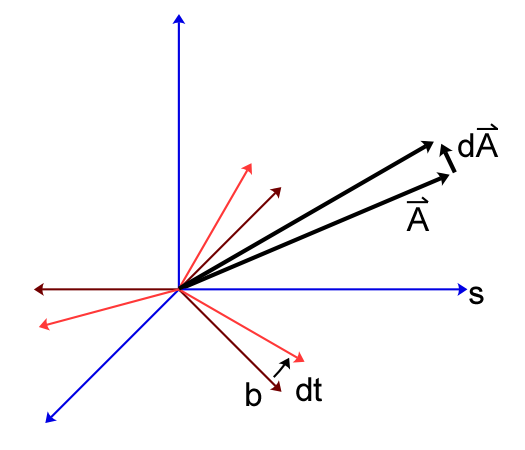
\includegraphics[scale=0.7]{vecratechange.JPG}}
\end{center}
\end{figure}

\bigskip \U{5728}\U{6642}\U{9593}t\U{6642}\U{6211}\U{5011}\U{4ee4}S\U{8207}b
frame\U{91cd}\U{5408}\U{ff0c}\U{904e}\U{4e86}dt\U{6642}\U{9593}\U{539f}%
\U{672c}\U{7684}$\vec{A}$\U{5411}\U{91cf}\U{52a0}\U{4e86}\U{4e00}\U{6539}%
\U{8b8a}\U{91cf}$d\vec{A}$\U{ff0c}\U{4e26}\U{4e14}b frame\U{4f9d}\U{53f3}%
\U{624b}\U{5b9a}\U{5247}\U{8f49}\U{52d5}\U{4e86}\U{4e00}\U{5fae}\U{5c0f}%
\U{89d2}\U{5ea6}(infinitisemal rotation)\U{ff0c}\U{9019}\U{908a}\U{8003}%
\U{616e}\U{76f8}\U{540c}\U{7684}\U{65b9}\U{4fbf}\U{6027}\U{6211}\U{5011}%
\U{5047}\U{5b9a}$S_{x}$\U{8207}$b_{x}$\U{91cd}\U{548c}\U{ff0c}\U{4f46}%
\U{6240}\U{6709}\U{63a8}\U{5c0e}\U{5747}\U{8003}\U{616e}\U{6700}\U{4e00}%
\U{822c}\U{6027}\U{3002}\U{5728}\U{6b64}\U{524d}\U{63d0}\U{4e0b}\U{ff0c}%
\U{5411}\U{91cf}$\vec{A}$\U{5728}t\U{5230}t+dt\U{6642}\U{9593}\U{7686}%
\U{7b26}\U{5408}%
\begin{equation*}
\left( \vec{A}\right) _{s}=\left( \vec{A}\right) _{b}
\end{equation*}%
\U{63a5}\U{8457}\U{ff0c}\U{5728}t+dt\U{6642}\U{9593}$\vec{A}+d\vec{A}$%
\U{5411}\U{91cf}\U{5728}s\U{8207}b frame\U{9593}\U{7684}\U{95dc}\U{4fc2}%
\U{70ba}%
\begin{equation*}
\left( \vec{A}+d\vec{A}\right) _{b}=\underset{\text{passive, r.h.}}{\Omega }%
\left( \vec{A}+d\vec{A}\right) _{s}
\end{equation*}%
$\Omega $\U{70ba}s, b frame\U{8f49}\U{52d5}\U{77e9}\U{9663}(passive r.h.)%
\U{ff0c}\U{6b64}$\Omega $\U{77e9}\U{9663}\U{8207}\U{4e0a}\U{4e00}\U{6bb5}$%
\vec{A}$\U{4e0d}\U{8b8a}\U{52d5}\U{7684}\U{60c5}\U{6cc1}\U{7684}$\Omega $%
\U{77e9}\U{9663}\U{5b8c}\U{5168}\U{76f8}\U{540c}\U{ff0c}\U{6211}\U{5011}%
\U{53d6}s\U{5230}b frame\U{7684}\U{8f49}\U{52d5}\U{70ba}\U{5fae}\U{5c0f}%
\U{91cf}\U{ff0c}$\Omega \rightarrow d\Omega $\U{ff0c}\U{4e0a}\U{5f0f}\U{4f9d}%
\U{4e4b}\U{524d}\U{6240}\U{8ff0}\U{7684}\U{539f}\U{7406}\U{53ef}\U{5beb}%
\U{6210}%
\begin{equation*}
\left( \vec{A}+d\vec{A}\right) _{b}=\underset{\text{passive, r.h.}}{\left(
1+\epsilon \right) }\left( \vec{A}+d\vec{A}\right) _{s}
\end{equation*}%
\U{8981}\U{5f37}\U{8abf}\U{9019}\U{908a}\U{7684}$\epsilon $\U{77e9}\U{9663}%
\U{8ddf}\U{4e4b}\U{524d}\U{4e0a}\U{4e00}\U{6bb5}\U{7684}$\epsilon $\U{77e9}%
\U{9663}\U{662f}\U{5b8c}\U{5168}\U{76f8}\U{540c}\U{7684}\U{ff0c}\U{5c55}%
\U{958b}\U{4e0a}\U{5f0f}%
\begin{equation*}
\left( \vec{A}\right) _{b}+\left( d\vec{A}\right) _{b}=\left( \vec{A}\right)
_{s}+\left( d\vec{A}\right) _{s}+\epsilon \left( \vec{A}\right)
_{s}+\epsilon \left( d\vec{A}\right) _{s}
\end{equation*}%
\U{5229}\U{7528}\U{4e4b}\U{524d}\U{77e5}\U{9053}\U{7684}$\left( \vec{A}%
\right) _{s}=\left( \vec{A}\right) _{b}$\U{ff0c}\U{4ee5}\U{53ca}\U{5ffd}%
\U{7565}\U{9ad8}\U{968e}\U{9805}$\epsilon \left( d\vec{A}\right) _{s}$%
\U{ff0c}\U{91cd}\U{65b0}\U{6574}\U{7406}\U{6210}%
\begin{equation*}
\left( d\vec{A}\right) _{s}=\left( d\vec{A}\right) _{b}-\underset{\text{r.h.}%
}{\epsilon }\left( \vec{A}\right) _{s}
\end{equation*}%
\U{4f9d}\U{4e4b}\U{524d}\U{6240}\U{8ff0}\U{539f}\U{7406}\U{4ee3}\U{5165}r.h. 
$\epsilon $\U{7684}\U{516c}\U{5f0f}\U{ff0c}\U{4e26}\U{4e14}\U{5229}\U{7528}%
\U{5411}\U{91cf}\U{5916}\U{7a4d}%
\begin{eqnarray*}
\left( d\vec{A}\right) _{s} &=&\left( d\vec{A}\right) _{b}-\left[ 
\begin{array}{ccc}
0 & \epsilon _{3}\geq 0 & -\epsilon _{2}\leq 0 \\ 
-\epsilon _{3} & 0 & \epsilon _{1}\geq 0 \\ 
\epsilon _{2} & -\epsilon _{1} & 0%
\end{array}%
\right] \left( \vec{A}\right) _{s} \\
&=&\left( d\vec{A}\right) _{b}-\left( \vec{A}\right) _{s}\times \left( d\vec{%
\Omega}\right) _{s} \\
&=&\left( d\vec{A}\right) _{b}+\left( d\vec{\Omega}\right) _{s}\times \left( 
\vec{A}\right) _{s}
\end{eqnarray*}%
\U{56e0}\U{70ba}\U{9019}\U{88e1}\U{7684}$\epsilon $\U{77e9}\U{9663}\U{8207}%
\U{4e0a}\U{4e00}\U{6bb5}\U{7684}$\epsilon $\U{77e9}\U{9663}\U{662f}\U{4e00}%
\U{6a23}\U{7684}\U{ff0c}\U{56e0}\U{6b64}\U{6211}\U{5011}\U{4e5f}\U{53ef}%
\U{4ee5}\U{7528}\U{4e0a}\U{4e4b}\U{524d}\U{8f49}\U{52d5}\U{516c}\U{5f0f}%
\U{6240}\U{63a8}\U{5c0e}\U{7684}\U{5fae}\U{5c0f}\U{8f49}\U{52d5}\U{77e9}%
\U{9663}$\epsilon $\U{6240}\U{5c0d}\U{61c9}\U{7684}\U{8f49}\U{52d5}\U{5411}%
\U{91cf}$\left( d\vec{\Omega}\right) $\U{ff0c}\U{9019}\U{6a23}\U{6211}%
\U{5011}\U{5c31}\U{5f97}\U{5230}\U{4e86}rate of change of a vector in
rotating frame\U{516c}\U{5f0f}%
\begin{equation}
\left( d\vec{A}\right) _{s}=\left( d\vec{A}\right) _{b}+\left( d\vec{\Omega}%
\right) _{s}\times \left( \vec{A}\right) _{s}  \label{rateofdomega}
\end{equation}%
\U{9019}\U{908a}\U{8981}\U{5f37}\U{8abf}\U{ff0c}\U{56e0}\U{70ba}\U{9019}%
\U{88e1}\U{7684}$\epsilon $\U{77e9}\U{9663}\U{8207}\U{4e0a}\U{4e00}\U{6bb5}%
\U{7684}$\epsilon $\U{77e9}\U{9663}\U{662f}\U{4e00}\U{6a23}\U{7684}\U{ff0c}%
\U{6240}\U{4ee5}\U{8b49}\U{660e}\U{4e86}$d\vec{\Omega}$\U{6240}\U{5c0d}%
\U{61c9}\U{7684}\U{5411}\U{91cf}\U{5c31}\U{662f}s frame\U{8f49}\U{5230}b
frame\U{7684}\U{89d2}\U{4f4d}\U{79fb}\U{5411}\U{91cf}(r.h.)\U{ff0c}\U{9019}%
\U{6a23}\U{5f37}\U{8abf}\U{7684}\U{76ee}\U{7684}\U{662f}\U{ff0c}\U{6211}%
\U{5011}\U{6703}\U{4ee5}\U{6b64}\U{7279}\U{6027}\U{6a21}\U{64ec}\U{525b}%
\U{9ad4}\U{8f49}\U{52d5}\U{3002}\U{53e6}\U{5916}\U{8981}\U{6ce8}\U{610f}%
\U{7684}\U{662f}$\vec{A}$\U{8207}$d\vec{\Omega}$\U{662f}\U{6cbf}\U{8457}t%
\U{6642}\U{9593}\U{7684}s frame\U{53d6}\U{7684}\U{6295}\U{5f71}\U{91cf}%
\U{3002}\U{9019}\U{908a}\U{503c}\U{5f97}\U{4e00}\U{63d0}\U{7684}\U{662f}%
\U{ff0c}\U{50b3}\U{7d71}\U{516c}\U{5f0f}\U{5927}\U{591a}\U{5beb}\U{6210}%
\begin{equation*}
\left( d\vec{A}\right) _{s}=\left( d\vec{A}\right) _{b}+\left( d\vec{\Omega}%
\right) _{b}\times \left( \vec{A}\right) _{b}
\end{equation*}%
\U{9019}\U{908a}$\vec{A}$\U{8207}$d\vec{\Omega}$\U{5247}\U{662f}\U{6cbf}%
\U{8457}t+dt\U{6642}\U{9593}\U{7684}b frame\U{53d6}\U{7684}\U{6295}\U{5f71}%
\U{91cf}\U{ff0c}\U{56e0}\U{82e5}\U{8003}\U{616e}$\left( \vec{A}\right) _{b}$%
\U{90a3}\U{6211}\U{5011}\U{7684}\U{5fae}\U{5c0f}\U{77e9}\U{9663}\U{662f}%
\U{4f5c}\U{7528}\U{5728}body frame\U{7684}$\vec{A}$\U{4e0a}\U{9762}\U{ff0c}%
\U{56e0}\U{6b64}\U{5728}\U{5229}\U{7528}\U{5916}\U{7a4d}\U{7279}\U{6027}%
\U{4f86}\U{6307}\U{5b9a}\U{8f49}\U{52d5}\U{5411}\U{91cf}\U{6642}\U{6211}%
\U{5011}\U{4e5f}\U{8003}\U{616e}$\left( d\vec{\Omega}\right) _{b}$\U{5728}b
frame\U{7684}\U{6295}\U{5f71}$\U{ff0c} $\U{56e0}\U{6b64}\U{4e8b}\U{5be6}%
\U{4e0a}$\vec{A}$\U{8207}$d\vec{\Omega}$\U{53d6}s\U{6216}b frame\U{5206}%
\U{91cf}\U{90fd}\U{662f}\U{53ef}\U{4ee5}\U{7684}\U{ff0c}\U{53ea}\U{8981}%
\U{77e9}\U{9663}\U{904b}\U{7b97}\U{5f8c}\U{51fa}\U{4f86}\U{7684}\U{7d50}%
\U{679c}\U{662f}\U{4e00}\U{6a23}\U{7684}\U{5c31}\U{53ef}\U{4ee5}\U{3002}%
\footnote{%
Goldstein\U{5728}\U{66f8}\U{4e0a}\U{5728}\U{9019}\U{90e8}\U{5206}\U{7684}%
\U{8aaa}\U{660e}\U{6bd4}\U{8f03}\U{5c11}\U{ff0c}\U{4e0d}\U{904e}\U{4ed6}%
\U{4e5f}\U{63d0}\U{5230}\U{53ea}\U{8981}\U{5728}\U{5fae}\U{5206}\U{53d6}%
\U{5b8c}\U{5f8c}\U{ff0c}\U{5411}\U{91cf}\U{6cbf}space\U{6216}body\U{53d6}%
\U{5206}\U{91cf}\U{90fd}\U{662f}\U{53ef}\U{4ee5}\U{7684}\cite[p. 176]%
{goldstein}\U{3002}}

\bigskip \U{4e0a}\U{5f0f}\U{53d6}\U{5fae}\U{5206}\U{5373}\U{5f97}\U{5230}%
\U{4e00}\U{822c}\U{5e38}\U{898b}\U{7684}\U{5f62}\U{5f0f}%
\begin{equation}
\left( \frac{d\vec{A}}{dt}\right) _{s}=\left( \frac{d\vec{A}}{dt}\right)
_{b}+\left( \vec{\omega}\right) _{s}\times \left( \vec{A}\right) _{s}
\label{rateofchange}
\end{equation}%
\U{5176}\U{4e2d}$\left( \vec{\omega}\right) _{s}$\U{70ba}s frame\U{5230}b
frame\U{7684}\U{77ac}\U{6642}\U{89d2}\U{901f}\U{5ea6}\U{3002}

\U{56b4}\U{8b39}\U{7684}\U{5b9a}\U{7fa9}\U{4e86}$d\vec{\Omega}$\U{8207}$%
\left( \vec{\omega}\right) _{s}$\U{5f8c}\U{ff0c}\U{6211}\U{5011}\U{63a5}%
\U{8457}\U{53ef}\U{4ee5}\U{5229}\U{7528}Calvin Klein parameter\U{4f86}%
\U{8fd1}\U{4f3c}\U{539f}\U{672c}\U{7684}\U{8f49}\U{52d5}\U{77e9}\U{9663}(%
\U{4e5f}\U{5c31}\U{662f}$1+\epsilon $\U{77e9}\U{9663}\U{ff0c}CK parameters%
\U{77e9}\U{9663}\U{662f}\U{5f9e}\U{8f49}\U{52d5}\U{5411}\U{91cf}\U{5efa}%
\U{7acb}\U{8f49}\U{52d5}\U{77e9}\U{9663}\U{7684}path order exponential%
\U{7684}\U{7b2c}\U{4e00}\U{968e}\U{8fd1}\U{4f3c}\U{ff0c}\U{8a73}\U{7d30}%
\U{63a8}\U{5c0e}\U{8acb}\U{53c3}\U{8003}\cite[p. 47\symbol{126}50]{tong}%
\U{ff0c}\U{4e4b}\U{5f8c}\U{6211}\U{4e5f}\U{5e0c}\U{671b}\U{80fd}\U{5920}%
\U{5617}\U{8a66}\U{66f4}\U{9ad8}\U{968e}\U{7684}\U{8fd1}\U{4f3c}\U{ff0c}%
\U{9019}\U{908a}\U{6211}\U{5011}\U{7d66}\U{4ed6}\U{4e00}\U{500b}\U{65b0}%
\U{4ee3}\U{865f}$CK(d\vec{\Omega})$\U{ff0c}\U{7576}\U{7136}\U{ff0c}\U{63a5}%
\U{4e0b}\U{4f86}\U{53ea}\U{8981}\U{662f}\U{77e9}\U{9663}\U{904b}\U{7b97}%
\U{6211}\U{5011}\U{90fd}\U{6703}\U{5beb}\U{4e0a}$CK$\U{7684}\U{4e3b}\U{88ab}%
\U{52d5}\U{53ca}\U{5de6}\U{53f3}\U{624b}\U{6027}\U{8cea}\footnote{\U{529b}%
\U{77e9}\U{7d66}\U{51fa}\U{7684}\U{89d2}\U{901f}\U{5ea6}\U{662f}\U{9075}%
\U{5b88}\U{53f3}\U{624b}\U{5b9a}\U{5247}(counterclockwise)\U{ff0c}\U{6240}%
\U{4ee5}CK\U{77e9}\U{9663}\U{5fc5}\U{9808}\U{4f7f}\U{7528}\U{5176}active
counterclockwise sense\U{624d}\U{80fd}\U{63cf}\U{8ff0}\U{6b63}\U{78ba}%
\U{5411}\U{91cf}\U{8f49}\U{52d5}\U{ff0c}\U{8981}\U{5c0f}\U{5fc3}\U{ff0c}%
\U{56e0}\U{5927}\U{90e8}\U{5206}\U{66f8}\U{4e0a}(\U{5982}Goldstein)\U{7d66}%
\U{7684}\U{516c}\U{5f0f}\U{90fd}\U{662f}active clockwise(follow\U{5de6}%
\U{624b}\U{5b9a}\U{5247})(\U{8209}\U{4f8b}\U{5982}\U{66f8}\U{4e0a}\U{7684}%
Caley Klein parameter rotation matrix)\U{ff0c}\U{56e0}\U{6b64}\U{5dee}%
\U{4e00}\U{500b}\U{8ca0}\U{865f}\U{3002}}\U{3002}%
\begin{eqnarray*}
\underset{\text{r.h.}}{CK(d\vec{\Omega})} &=&\left[ 
\begin{array}{ccc}
a^{2}+b^{2}-c^{2}-d^{2} & 2(bc-ad) & 2(bd+ac) \\ 
2(bc+ad) & a^{2}+c^{2}-b^{2}-d^{2} & 2(cd-ab) \\ 
2(bd-ac) & 2(cd+ab) & a^{2}+d^{2}-b^{2}-c^{2}%
\end{array}%
\right] \text{,} \\
\text{with }a &=&\cos \left( \frac{\left\vert d\vec{\Omega}\right\vert }{2}%
\right) \text{, b, c, d = component of }d\hat{\Omega}\cdot \sin \left( \frac{%
\left\vert d\vec{\Omega}\right\vert }{2}\right)
\end{eqnarray*}%
\U{73fe}\U{5728}\U{ff0c}\U{6211}\U{5011}\U{4e00}\U{518d}\U{5f37}\U{8abf}$d%
\vec{\Omega}$\U{6240}\U{5c0d}\U{61c9}\U{7684}\U{662f}s frame\U{8f49}\U{52d5}%
\U{5230}b frame\U{ff0c}\U{56e0}\U{6b64}\U{6211}\U{5011}\U{5efa}\U{7acb}%
\U{7684}$CK(d\vec{\Omega})$\U{77e9}\U{9663}\U{5177}\U{6709}\U{4ee5}\U{4e0b}%
\U{7684}\U{7279}\U{6027}\U{ff0c}\U{6839}\U{64da}\U{5716}\ref{ratevecfig}%
\U{ff0c}%
\begin{eqnarray*}
\left( \vec{A}\right) _{b} &=&\underset{\text{passive, r.h.}}{CK(d\vec{\Omega%
})}\left( \vec{A}\right) _{s} \\
\left( \hat{S}_{y}\right) _{s} &=&\underset{\text{active, l.h.}}{CK(d\vec{%
\Omega})}\left( \hat{b}_{y}\right) _{s}
\end{eqnarray*}%
\U{6216}\U{8005}%
\begin{eqnarray}
\left( \vec{A}\right) _{s} &=&\underset{\text{active, l.h.}}{\underbrace{%
\left[ CK(d\vec{\Omega})\right] ^{T}}}\left( \vec{A}\right) _{b}
\label{frametrans} \\
\left( \hat{b}_{y}\right) _{s} &=&\underset{\text{active, r.h.}}{\underbrace{%
\left[ CK(d\vec{\Omega})\right] ^{T}}}\left( \hat{S}_{y}\right) _{s}
\label{vecrot}
\end{eqnarray}%
\ref{ratevecfig}\U{82e5}\U{6211}\U{5011}\U{77e5}\U{9053}\U{7684}\U{662f}$%
\left( \vec{\omega}\right) _{s}$\U{5247}\U{53ef}\U{5e36}\U{5165}$CK(\left( 
\vec{\omega}\right) _{s}\cdot dt)$\U{4f86}\U{5f97}\U{5230}\U{77e9}\U{9663}%
\U{3002}\U{4ee5}\U{4e0a}\U{5169}\U{5f0f}\U{5c31}\U{662f}\U{6a21}\U{64ec}%
\U{6216}\U{8ffd}\U{8e64}\U{525b}\U{9ad4}\U{7684}body frame\U{7684}x,y,z%
\U{8ef8}\U{8f49}\U{52d5}\U{7684}\U{57fa}\U{790e}\U{3002}

\begin{figure}[th]
\caption{How to apply rate-of-change-of-a-vector equation to a real
rotation. }
\label{szsbtdtfig}
\begin{center}
\fbox{\includegraphics[scale=0.7]{szsbtdt.JPG}}
\end{center}
\end{figure}

\U{5728}\U{6211}\U{5011}\U{9032}\U{4e00}\U{6b65}\U{8a0e}\U{8ad6}\ref%
{frametrans}\U{53ca}\ref{vecrot}\U{5f0f}\U{524d}\U{ff0c}\U{6211}\U{5011}%
\U{5fc5}\U{9808}\U{5148}\U{8aaa}\U{660e}\U{6211}\U{5011}\U{5982}\U{4f55}%
\U{61c9}\U{7528}\U{4e0a}\ref{rateofchange}\U{5f0f}\U{4f86}\U{89e3}\U{525b}%
\U{9ad4}\U{8f49}\U{52d5}\U{3002}\U{6211}\U{5011}\U{6703}\U{628a}\U{525b}%
\U{9ad4}\U{8f49}\U{52d5}\U{5206}\U{89e3}\U{70ba}\U{5f88}\U{591a}\U{7684}%
\U{5fae}\U{5c0f}\U{8f49}\U{52d5}\U{ff0c}\U{6bcf}\U{4e00}\U{5c0f}\U{6bb5}%
\U{7684}\U{5fae}\U{5c0f}\U{8f49}\U{52d5}\U{6211}\U{5011}\U{90fd}\U{6703}%
\U{904b}\U{7528}\U{4e0a}\U{5716}\ref{ratevecfig}\U{7684}\U{539f}\U{7406}%
\U{ff0c}\U{73fe}\U{5728}\U{6211}\U{5011}\U{9700}\U{8981}\U{53e6}\U{5916}%
\U{8a2d}\U{5b9a}\U{4e00}\U{500b}Lab frame\thinspace \U{ff0c}\U{898b}\U{5716}%
\ref{szsbtdtfig}\U{ff0c}\U{6b64}\U{70ba}\U{771f}\U{6b63}\U{7684}\U{89c0}%
\U{6e2c}\U{8005}\U{6240}\U{8655}\U{5728}\U{7684}inertial frame\U{3002}%
\U{8003}\U{616e}\U{4efb}\U{610f}\U{4e00}\U{6bb5}\U{5fae}\U{5c0f}\U{8f49}%
\U{52d5}t\U{5230}t+dt\U{ff0c}\U{5728}t\U{6642}\U{523b}\U{6642}\U{6211}%
\U{5011}\U{5c07}\U{525b}\U{9ad4}\U{7684}principle axes\U{8a2d}\U{5b9a}%
\U{70ba}S frame\U{ff0c}\U{518d}\U{5c07}t+dt\U{6642}\U{523b}\U{525b}\U{9ad4}%
\U{7684}principle axes\U{8a2d}\U{5b9a}\U{70ba}b frame\U{ff0c}\U{9019}\U{6a23}%
\U{4ee3}\U{8868}s frame\U{5230}b frame\U{5c31}\U{662f}\U{525b}\U{9ad4}t%
\U{5230}t+dt\U{7684}\U{8f49}\U{52d5}\U{3002}\U{5c07}\ref{rateofchange}%
\U{5f0f}\U{61c9}\U{7528}\U{4e0a}\U{9019}\U{4e00}\U{6bb5}t\U{5230}t+dt\U{7684}%
\U{5fae}\U{5c0f}\U{8f49}\U{52d5}\U{ff0c}\U{4e26}\U{4e14}\U{8003}\U{616e}$%
\vec{A}$\U{70ba}\U{525b}\U{9ad4}\U{89d2}\U{52d5}\U{91cf}$\vec{L}$\U{ff0c}%
\U{5247}\U{6211}\U{5011}\U{5f97}\U{5230}%
\begin{equation}
\left( \Gamma \right) _{s}=\left( \frac{d\vec{L}}{dt}\right) _{s}=\left( 
\frac{d\vec{L}}{dt}\right) _{b}+\left( \vec{\omega}\right) _{s}\times \left( 
\vec{L}\right) _{s}  \label{liw}
\end{equation}%
\U{9019}\U{88e1}\U{7b2c}\U{4e00}\U{7b49}\U{865f}\U{4e5f}\U{7528}\U{4e0a}%
\U{725b}\U{9813}\U{5b9a}\U{5f8b}\U{3002}\U{73fe}\U{5728}\U{6211}\U{5011}%
\U{5f9e}\ref{rateofdomega}\U{5f0f}\U{77e5}\U{9053}$\left( d\vec{\Omega}%
\right) _{s}$\U{662f}s\U{5230}b frame\U{7684}\U{89d2}\U{4f4d}\U{79fb}\U{ff0c}%
\U{800c}\U{9019}\U{908a}\U{7d93}\U{7531}\U{6211}\U{5011}\U{7684}\U{8a2d}%
\U{5b9a}\U{ff0c}s\U{5230}b frame\U{6b63}\U{662f}\U{6211}\U{5011}\U{525b}%
\U{9ad4}\U{7279}\U{5fb5}\U{8ef8}\U{5f9e}t\U{5230}t+dt\U{7684}\U{89d2}\U{4f4d}%
\U{79fb}\U{ff0c}\U{56e0}\U{6b64}$\left( \frac{d\vec{\Omega}}{dt}\right)
_{s}=\left( \vec{\omega}\right) _{s}$\U{6b63}\U{662f}\U{525b}\U{9ad4}\U{7684}%
\U{77ac}\U{6642}\U{89d2}\U{901f}\U{5ea6}(\U{6cbf}\U{8457}t\U{6642}\U{9593}s
frame\U{53d6}\U{5206}\U{91cf})\U{ff0c}\U{63a5}\U{8457}\U{ff0c}\U{56e0}%
\U{70ba}s, b frame\U{90fd}\U{662f}\U{6cbf}\U{8457}body principle axes\U{800c}%
\U{53d6}\U{ff0c}\U{56e0}\U{6b64}\U{6cbf}s frame\U{7684}\U{89d2}\U{52d5}%
\U{91cf}$\left( \vec{L}\right) _{s}$\U{53ef}\U{4ee5}\U{5beb}\U{6210}%
\begin{equation*}
\left( \vec{L}\right) _{s}=\left[ 
\begin{array}{ccc}
I_{xx} & 0 & 0 \\ 
0 & I_{yy} & 0 \\ 
0 & 0 & I_{zz}%
\end{array}%
\right] \times \left( \vec{\omega}\right) _{s}
\end{equation*}%
\U{518d}\U{6b21}\U{6ce8}\U{610f}$\left( \Gamma \right) _{s}$\U{8207}$\left( 
\vec{\omega}\right) _{s}$\U{8207}$\left( \vec{L}\right) _{s}$\U{90fd}\U{662f}%
\U{6cbf}\U{8457}t\U{6642}\U{523b}\U{7684}\U{525b}\U{9ad4}\U{7279}\U{5fb5}%
\U{8ef8}(\U{4e5f}\U{5c31}\U{662f}s frame)\U{53d6}\U{7684}\U{6295}\U{5f71}%
\U{ff0c}\U{4e26}\U{4e0d}\U{662f}Lab frame\U{7684}\U{6295}\U{5f71}\U{ff0c}%
\U{9019}\U{9ede}\U{8981}\U{7279}\U{5225}\U{6ce8}\U{610f}\U{ff0c}\U{57fa}%
\U{672c}\U{4e0a}\U{9019}\U{4ee3}\U{8868}\U{ff0c}$\left( \vec{\omega}\right)
_{s}$\U{5c31}\U{662f}\U{8cbc}\U{9ad4}\U{89d2}\U{901f}\U{5ea6}\U{ff01}\U{4e26}%
\U{4e14}$\left( \Gamma \right) _{s}$\U{662f}\U{8cbc}\U{9ad4}\U{7684}\U{89d2}%
\U{52d5}\U{91cf}\U{ff01}\U{9019}\U{88e1}\U{5927}\U{90e8}\U{5206}\U{7684}%
\U{66f8}\U{4e0a}\U{90fd}\U{6c92}\U{6709}\U{7d66}\U{51fa}\U{6070}\U{7576}%
\U{7684}\U{539f}\U{56e0}\footnote{\U{6ce8}\U{610f}\U{56e0}\U{70ba}s frame%
\U{6703}\U{6301}\U{7e8c}\U{7684}\U{6539}\U{8b8a}\U{6240}\U{4ee5}$\left( \vec{%
\Gamma}\right) _{s}$\U{4e0d}\U{53ef}\U{53d6}$\left( \vec{\Gamma}\right)
_{lab}$\U{7684}\U{503c}\U{ff0c}\U{540c}\U{7406}$\left( \vec{\omega}\right)
_{s}$\U{4e5f}\U{4e0d}\U{662f}$\left( \vec{\omega}\right) _{lab}$\U{ff0c}%
\U{5169}\U{8005}\U{90fd}\U{5fc5}\U{9808}\U{7d93}\U{904e}\U{8f49}\U{63db}%
\U{5f9e}lab\U{8f49}\U{5230}t\U{6642}\U{523b}s frame\U{3002}}\U{3002}\U{9019}%
\U{908a}\U{6211}\U{5011}\U{8b49}\U{660e}\U{4e86}\ref{liw}\U{5f0f}\U{6700}%
\U{5f8c}\U{90a3}\U{4e00}\U{9805}\U{4e2d}\U{7684}\U{5169}\U{500b}$\vec{\omega}
$\U{662f}\U{76f8}\U{540c}\U{7684}\footnote{\U{4f46}\U{6211}\U{5011}\U{5fc5}%
\U{9808}\U{5f37}\U{8abf}\U{ff0c}\U{4efb}\U{610f}\U{60c5}\U{6cc1}\U{4e0b}%
\U{ff0c}\U{89d2}\U{901f}\U{5ea6}$\left( \vec{\omega}\right) $\U{5728}body%
\U{8f49}\U{52d5}\U{5ea7}\U{6a19}\U{4e0b}\U{7684}\U{6295}\U{5f71}\U{4e26}%
\U{4e0d}\U{662f}body\U{5ea7}\U{6a19}\U{4e0a}\U{89c0}\U{5bdf}\U{5230}\U{7684}%
\U{89d2}\U{901f}\U{5ea6}\U{ff01}\U{9019}\U{662f}\U{5f88}\U{5e38}\U{898b}%
\U{7684}\U{932f}\U{8aa4}\U{ff0c}\U{9019}\U{88e1}\U{6211}\U{5011}\U{662f}%
\U{6709}\U{689d}\U{4ef6}\U{7684}\U{8003}\U{616e}t\U{5230}t+dt\U{6642}\U{523b}%
\U{7684}t\U{6642}\U{523b}s,b\U{5ea7}\U{6a19}\U{91cd}\U{548c}\U{3002}}\U{3002}%
\U{4e26}\U{4e14}\U{ff0c}\U{529b}\U{77e9}\U{4e5f}\U{5fc5}\U{9808}\U{5f9e}lab
frame\U{8f49}\U{63db}\U{5230}t\U{6642}\U{9593}\U{7684}s frame\U{3002}\U{4ee3}%
\U{5165}$\vec{L}$\U{4e26}\U{5c55}\U{958b}\ref{liw}\U{5f0f}\U{ff0c}\U{6211}%
\U{5011}\U{5c31}\U{5f97}\U{5230}\U{6240}\U{8b02}\U{7684}\U{5c24}\U{62c9}%
\U{516c}\U{5f0f}(Euler's equation)%
\begin{eqnarray}
\Gamma _{x}(t) &=&I_{x}\dot{\omega}_{x}+(I_{z}-I_{y})\omega _{y}\left(
t\right) \omega _{z}\left( t\right)  \notag \\
\Gamma _{y}(t) &=&I_{y}\dot{\omega}_{y}+(I_{x}-I_{z})\omega _{x}\omega _{z}
\label{eulereqbody} \\
\Gamma _{z}(t) &=&I_{z}\dot{\omega}_{z}+(I_{x}-I_{y})\omega _{x}\omega _{y} 
\notag
\end{eqnarray}%
\U{6ce8}\U{610f}$\vec{\Gamma}$\U{53ca}$\vec{\omega}$\U{7684}x,y,z\U{5206}%
\U{91cf}\U{90fd}\U{662f}\U{6cbf}\U{8457}t\U{6642}\U{523b}\U{7684}\U{525b}%
\U{9ad4}\U{7279}\U{5fb5}\U{8ef8}s frame\U{53d6}\U{7684}\U{5206}\U{91cf}%
\U{ff0c}\U{9019}\U{9ede}\U{5fc5}\U{9808}\U{8981}\U{5f37}\U{8abf}\U{3002}%
\U{4e4b}\U{5f8c}\U{6578}\U{503c}\U{6a21}\U{64ec}\U{7684}\U{6642}\U{5019}%
\U{9019}\U{9ede}\U{662f}\U{91cd}\U{8981}\U{7684}\U{3002}

\U{6211}\U{5011}\U{5c07}\U{5728}\U{525b}\U{9ad4}\U{7279}\U{5fb5}\U{8ef8}%
\U{7684}\U{6bcf}\U{4e00}\U{6bb5}t\U{5230}t+dt\U{7684}\U{5206}\U{89e3}\U{904b}%
\U{52d5}\U{904b}\U{7528}\U{4e0a}s frame\U{8f49}\U{5230}b frame\U{7684}%
\U{5c24}\U{62c9}\U{516c}\U{5f0f}\U{ff0c}\U{4e5f}\U{5c31}\U{662f}\U{904b}%
\U{7528}\U{4e0a}\ref{eulereqbody}\U{5f0f}\U{3002}\U{9019}\U{4e5f}\U{4ee3}%
\U{8868}\U{6211}\U{5011}\U{5c07}\U{6301}\U{7e8c}\U{5730}\U{6539}\U{8b8a}%
space frame\U{4f86}\U{7b26}\U{5408}\U{9019}\U{500b}\U{689d}\U{4ef6}\U{ff0c}%
\U{4f46}\U{662f}\U{7576}\U{7136}\U{6211}\U{5011}\U{6703}\U{8ddf}\U{8e64}%
space frame\U{6bcf}\U{4e00}\U{500b}\U{8b8a}\U{63db}\U{7684}\U{4f4d}\U{7f6e}%
\U{4f86}\U{9054}\U{5230}\U{6a21}\U{64ec}\U{8f49}\U{52d5}\U{904b}\U{52d5}%
\U{ff0c}\U{800c}\U{9019}\U{6642}\U{5019}\U{5c31}\U{6703}\U{7528}\U{4e0a}\ref%
{frametrans}\U{53ca}\ref{vecrot}\U{5f0f}\U{3002}

\U{63a5}\U{4e0b}\U{4f86}\U{61c9}\U{7528}\U{4e0a}\U{9640}\U{87ba}\U{ff0c}%
\U{82e5}\U{8003}\U{616e}\U{9640}\U{87ba}\U{7684}\U{689d}\U{4ef6} $%
I_{x}=I_{y}\neq I_{z}$\U{ff0c}\ref{eulereqbody}\U{5f0f}\U{53ef}\U{5beb}%
\U{6210}%
\begin{equation}
\frac{d}{dt}\left[ 
\begin{array}{c}
\omega _{x} \\ 
\omega _{y} \\ 
\omega _{z}%
\end{array}%
\right] =\left[ 
\begin{array}{ccc}
0 & -\frac{I_{z}-I_{y}}{I_{x}} & 0 \\ 
-\frac{I_{x}-I_{z}}{I_{y}} & 0 & 0 \\ 
0 & 0 & 0%
\end{array}%
\right] \left[ 
\begin{array}{c}
\omega _{x} \\ 
\omega _{y} \\ 
\omega _{z}%
\end{array}%
\right] +\left[ 
\begin{array}{c}
\frac{\Gamma _{x}}{I_{x}} \\ 
\frac{\Gamma _{y}}{I_{y}} \\ 
\frac{\Gamma _{z}}{I_{z}}%
\end{array}%
\right]
\end{equation}%
\U{5982}\U{4e4b}\U{524d}\U{6240}\U{5f37}\U{8abf}\U{ff0c}\U{53f3}\U{908a}%
\U{6240}\U{6709}\U{9805}\U{90fd}\U{662f}\U{5728}\U{6642}\U{9593}\U{70ba}t%
\U{6642}\U{523b}\U{7684}s frame\U{53d6}\U{5f97}\U{503c}\U{ff0c}\U{4e5f}%
\U{56e0}\U{6b64}\U{4ee5}\U{4e0a}\U{7684}\U{5fae}\U{5206}\U{65b9}\U{7a0b}%
\U{7d44}\U{53ef}\U{4ee5}\U{7528}\U{666e}\U{901a}\U{6578}\U{503c}\U{7531}%
\U{62c9}\U{6cd5}\U{6216}\U{56db}\U{968e}Ruge Kutta\U{6c42}\U{51fa}\U{5de6}%
\U{5074}$\omega _{x,y,z}(t+dt)$\U{ff0c}\U{4e5f}\U{5c31}\U{662f}\U{5f9e}$\vec{%
\omega}_{s}(t)$\U{6c42}\U{5f97}$\vec{\omega}_{s}(t+dt)$\U{3002}\U{4e0d}%
\U{904e}\U{5c0d}\U{65bc}\U{4efb}\U{610f}\U{7684}\U{525b}\U{9ad4}\U{8f49}%
\U{52d5}\U{7cfb}\U{7d71}\U{ff0c}\U{53ea}\U{8981}\U{80fd}\U{5f9e}\ref%
{eulereqbody}\U{5f0f}\U{53f3}\U{5074}$\vec{\omega}_{s}(t)$\U{6c42}\U{5f97}%
\U{5de6}\U{5074}$\vec{\omega}_{s}(t+dt)$\U{ff0c}\U{90fd}\U{9084}\U{662f}%
\U{80fd}\U{5920}\U{9069}\U{7528}\U{63a5}\U{4e0b}\U{4f86}\U{7684}\U{6a21}%
\U{64ec}\U{65b9}\U{6cd5}\U{ff0c}\U{6709}\U{4e0d}\U{5c11}\U{7684}\U{6578}%
\U{503c}\U{65b9}\U{6cd5}\U{53ef}\U{4ee5}\U{89e3}\U{4e00}\U{822c}\U{7684}%
\U{975e}\U{7dda}\U{6027}\U{4e00}\U{968e}ODE\U{5c24}\U{62c9}\U{65b9}\U{7a0b}%
\cite{matlab}\U{3002}

\U{73fe}\U{5728}\U{6211}\U{5011}\U{90fd}\U{8a2d}\U{5b9a}\U{597d}\U{4e86}%
\U{ff0c}\U{6211}\U{5011}\U{4e5f}\U{8b49}\U{660e}\U{4e86}\U{8cbc}\U{9ad4}%
\U{89d2}\U{901f}\U{5ea6}\U{5728}\U{4efb}\U{610f}\U{4e00}\U{6bb5}t\U{5230}t+dt%
\U{7684}\U{6642}\U{9593}\U{4e2d}\U{4ee3}\U{8868}\U{7684}\U{610f}\U{7fa9}%
\U{ff0c}\U{63a5}\U{4e0b}\U{4f86}\U{6211}\U{5011}\U{5c31}\U{8aaa}\U{660e}%
\U{5982}\U{4f55}\U{4ee5}\U{9019}\U{500b}\U{7279}\U{6027}\U{53ca}\U{5229}%
\U{7528}\ref{frametrans}\U{53ca}\ref{vecrot}\U{5f0f}\U{4f86}\U{8ffd}\U{8e64}%
s frame\U{5728}\U{5404}\U{500b}\U{5fae}\U{5c0f}\U{8f49}\U{52d5}\U{7684}%
\U{4f4d}\U{7f6e}\U{ff0c}\U{4e5f}\U{5c31}\U{662f}\U{6211}\U{5011}\U{8981}%
\U{6c42}\U{5f97}$\hat{S}_{x,y,z}(t_{i}$, i=1\symbol{126}N$)$ in the lab frame%
\U{3002}\bigskip \U{6211}\U{5011}\U{5c07}\U{4e0d}\U{5beb}\U{51fa}lab\U{7684}%
\U{4e0b}\U{6a19}\U{ff0c}\U{53ea}\U{8981}\U{6211}\U{5011}\U{8a18}\U{5f97}%
\U{6c92}\U{6709}\U{4e0b}\U{6a19}\U{5c31}\U{662f}\U{8868}\U{793a}\U{662f}lab
frame\U{3002}

\begin{figure}[th]
\caption{Boby\U{8ef8}\U{5728}\U{6bcf}\U{4e00}\U{5206}\U{6bb5}t\U{5230}t+dt%
\U{7684}\U{8ffd}\U{8e64}\U{793a}\U{610f}\U{5716}\U{3002}\U{6b64}\U{8655}%
\U{7684}$xyz_{s}$\U{61c9}\U{8a72}\U{662f}$xyz_{lab}$}
\begin{center}
\fbox{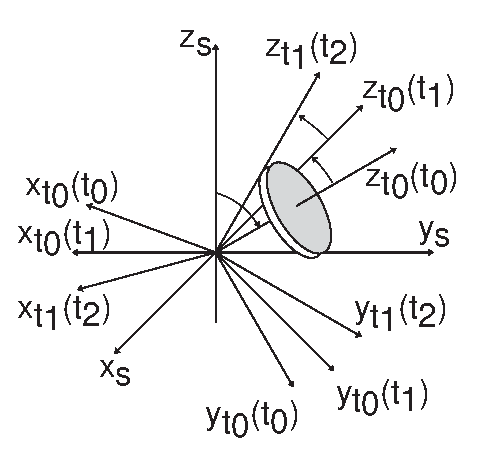
\includegraphics{top.eps}}
\end{center}
\end{figure}

\begin{figure}[th]
\caption{\U{9640}\U{87ba}\U{7684}\U{521d}\U{59cb}\U{503c}\U{8a2d}\U{5b9a}%
\U{3002}\U{6b64}\U{8655}\U{7684}$xyz_{s}$\U{61c9}\U{8a72}\U{662f}$xyz_{lab}$}
\begin{center}
\fbox{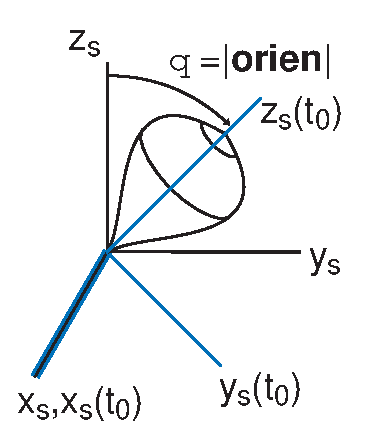
\includegraphics{initialsetup.eps}}
\end{center}
\end{figure}

\U{5047}\U{8a2d}\U{9640}\U{87ba}\U{7279}\U{5fb5}\U{8ef8}\U{5728}lab frame%
\U{7684}\U{8d77}\U{59cb}\U{4f4d}\U{7f6e}\U{5df2}\U{77e5}$\left( \hat{x}\hat{y%
}\hat{z}_{lab}(t_{0})\right) $\U{ff0c}\U{521d}\U{59cb}\U{8cbc}\U{9ad4}%
\U{89d2}\U{901f}\U{5ea6}\U{5df2}\U{77e5}$\vec{\omega}_{s}(t_{0})$\U{ff0c}%
\U{4e0b}\U{6a19}\U{4ee3}\U{8868}\U{7684}\U{662f}\U{89c0}\U{6e2c}\U{7684}frame%
\U{3002}\U{73fe}\U{5728}\U{6211}\U{5011}\U{5c07}s frame\U{653e}\U{5728}$%
\left( \hat{x}\hat{y}\hat{z}_{lab}(t_{0})\right) $\U{ff0c}\U{9019}\U{6a23}%
\U{4f9d}\U{7167}\U{5716}\ref{szsbtdtfig}\U{53ca}\U{5176}\U{6240}\U{8ff0}%
\U{539f}\U{7406}\U{ff0c}b frame\U{7684}\U{8ef8}\U{5c31}\U{662f}\U{6211}%
\U{5011}\U{8981}\U{6c42}\U{7684}$\left( \hat{x}\hat{y}\hat{z}%
_{lab}(t_{1})\right) $\U{ff0c}\U{82e5}\U{4ee5}$\hat{z}$\U{8ef8}\U{70ba}%
\U{4f8b}\U{ff0c}\ref{vecrot}\U{5f0f}\U{544a}\U{8a34}\U{6211}\U{5011}%
\begin{equation*}
\underset{\text{active, r.h.}}{\underbrace{\left[ CK\left( \vec{\omega}%
_{s}\left( t_{0}\right) dt\right) \right] ^{T}}}\times \hat{z}_{0}\left(
t_{0}\right) =\hat{z}_{0}\left( t_{1}\right)
\end{equation*}%
\U{5176}\U{4e2d}$\hat{z}_{0}\left( t_{0},t_{1}\right) $\U{4ee3}\U{8868}%
\U{6642}\U{9593}\U{70ba}$t_{0}$\U{8207}$t_{1}$\U{7684}\^{z}\U{8ef8}\U{5728}$%
t_{0}$\U{6642}\U{9593}\U{7684}\U{5ea7}\U{6a19}\U{8ef8}(\U{4e5f}\U{5c31}%
\U{662f}s frame)\U{7684}\U{6295}\U{5f71}\U{ff0c}\U{56e0}\U{6b64}$\hat{z}%
_{0}\left( t_{0}\right) $\U{70ba}\U{55ae}\U{4f4d}\U{5411}\U{91cf}$\left[ 
\begin{array}{ccc}
1 & 1 & 1%
\end{array}%
\right] $\U{3002}\U{9019}\U{6a23}\U{6211}\U{5011}\U{6c42}\U{5f97}\U{4e0b}%
\U{4e00}\U{500b}z\U{8ef8}\U{7684}\U{4f4d}\U{7f6e}\U{ff0c}\U{4e0d}\U{904e}%
\U{6211}\U{5011}\U{5f97}\U{8f49}\U{56de}lab frame\U{ff0c}\U{6211}\U{5011}%
\U{5047}\U{8a2d}lab frame\U{7684}xyz\U{8ef8}\U{5230}\U{9640}\U{87ba}\U{521d}%
\U{59cb}\U{4f4d}\U{7f6e}$\hat{x}\hat{y}\hat{z}_{lab}(t_{0})$\U{7684}\U{8f49}%
\U{52d5}\U{5411}\U{91cf}\U{662f}$\vec{\Omega}_{0}\U{ff0c} $\U{9019}\U{6a23}%
\U{6211}\U{5011}\U{53ef}\U{4ee5}\U{7528}$\vec{\Omega}_{0}$\U{8f15}\U{6613}%
\U{7684}\U{6539}\U{8b8a}\U{9640}\U{87ba}\U{521d}\U{59cb}\U{4f4d}\U{7f6e}%
\U{ff0c}\U{904b}\U{7528}\U{4e0a}\ref{frametrans}\U{5f0f}%
\begin{equation*}
\hat{z}_{lab}\left( t_{1}\right) =\underset{\text{passive, l.h.}}{%
\underbrace{\left[ CK\left( \vec{\Omega}_{0}\right) \right] ^{T}}}\times 
\hat{z}_{0}\left( t_{1}\right)
\end{equation*}%
\U{6ce8}\U{610f}\U{9019}\U{908a}\U{77e9}\U{9663}\U{5c31}\U{53d6}\U{88ab}%
\U{52d5}\U{542b}\U{610f}\U{ff0c}\U{7d50}\U{5408}\U{4ee5}\U{4e0a}\U{5169}%
\U{5f0f}\U{5f97}\U{5230}%
\begin{eqnarray*}
\hat{z}_{lab}\left( t_{1}\right) &=&\underset{\text{passive, l.h.}}{%
\underbrace{\left[ CK\left( \vec{\Omega}_{0}\right) \right] ^{T}}}\underset{%
\text{active, r.h.}}{\underbrace{\left[ CK\left( \vec{\omega}_{s}\left(
t_{0}\right) dt\right) \right] ^{T}}}\times \hat{z}_{0}\left( t_{0}\right) \\
&=&\underset{\text{passive, l.h.}}{\underbrace{\left[ CK\left( \vec{\Omega}%
_{0}\right) \right] ^{T}}}\underset{\text{active, r.h.}}{\underbrace{\left[
CK\left( \vec{\omega}_{s}\left( t_{0}\right) dt\right) \right] ^{T}}}\times %
\left[ 
\begin{array}{ccc}
1 & 1 & 1%
\end{array}%
\right]
\end{eqnarray*}%
\U{9019}\U{6a23}\U{6211}\U{5011}\U{5c31}\U{5f9e}t$_{0}$\U{6642}\U{9593}%
\U{5f97}\U{5230}t$_{1}$\U{6642}\U{9593}\U{9640}\U{87ba}z\U{8ef8}\U{7684}%
\U{4f4d}\U{7f6e}\U{3002}

\U{63a5}\U{8457}\U{82e5}\U{6211}\U{5011}\U{77e5}\U{9053}$\hat{z}_{lab}\left(
t_{i}\right) $\U{ff0c}\U{4ee5}\U{53ca}\U{5f9e}\U{5c24}\U{62c9}\U{516c}%
\U{5f0f}\U{6578}\U{503c}\U{6cd5}\U{89e3}\U{51fa}\U{7684}$\vec{\omega}%
_{s}\left( t_{0},t_{1},\cdots ,t_{i}\right) $\U{ff0c}\U{6211}\U{5011}\U{5716}%
\U{6a23}\U{53ef}\U{4ee5}\U{6c42}\U{5f97}$\hat{z}_{lab}\left( t_{i+1}\right) $%
\U{ff0c}\U{9996}\U{5148}\U{7528}\ref{vecrot}\U{5f0f}%
\begin{eqnarray*}
\hat{z}_{i}\left( t_{i+1}\right) &=&\underset{\text{active, r.h.}}{%
\underbrace{\left[ CK\left( \vec{\omega}_{s}\left( t_{i}\right) dt\right) %
\right] ^{T}}}\times \hat{z}_{i}\left( t_{i}\right) \\
&=&\underset{\text{active, r.h.}}{\underbrace{\left[ CK\left( \vec{\omega}%
_{s}\left( t_{i}\right) dt\right) \right] ^{T}}}\times \left[ 
\begin{array}{ccc}
1 & 1 & 1%
\end{array}%
\right]
\end{eqnarray*}%
\U{518d}\U{7528}\ref{frametrans}\U{5f0f}\U{8f49}\U{56de}\U{5230}lab frame%
\begin{eqnarray*}
\hat{z}_{lab}\left( t_{i+1}\right) &=&\underset{\text{passive, l.h.}}{%
\underbrace{\left[ CK\left( lab\rightarrow t_{i}\right) \right] ^{T}}}\times 
\hat{z}_{i}\left( t_{i+1}\right) \\
&=&\underset{\text{passive, l.h.}}{\underbrace{\left[ CK\left( \vec{\Omega}%
_{0}\right) \cdot CK\left( \vec{\omega}_{s}\left( t_{0}\right) dt\right)
\cdot CK\left( \vec{\omega}_{s}\left( t_{1}\right) dt\right) \cdot \cdots
\cdot CK\left( \vec{\omega}_{s}\left( t_{i-1}\right) dt\right) \right] ^{T}}}%
\times \\
&&\hat{z}_{i}\left( t_{i+1}\right) \\
&=&\underset{\text{passive, l.h.}}{\underbrace{\left[ CK\left( \vec{\Omega}%
_{0}\right) \cdot CK\left( \vec{\omega}_{s}\left( t_{0}\right) dt\right)
\cdot CK\left( \vec{\omega}_{s}\left( t_{1}\right) dt\right) \cdot \cdots
\cdot CK\left( \vec{\omega}_{s}\left( t_{i-1}\right) dt\right) \right] ^{T}}}%
\times \\
&&\underset{\text{active, r.h.}}{\underbrace{\left[ CK\left( \vec{\omega}%
_{s}\left( t_{i}\right) dt\right) \right] ^{T}}}\times \left[ 
\begin{array}{ccc}
1 & 1 & 1%
\end{array}%
\right]
\end{eqnarray*}%
\U{9019}\U{88e1}\U{7528}\U{4e0a}\U{4e0d}\U{540c}\U{6642}\U{9593}\U{5fae}%
\U{5c0f}\U{8f49}\U{52d5}\U{77e9}\U{9663}\U{7684}commutive\U{6027}\U{8cea}$%
\left( AB\right) C=A\left( BC\right) $\U{ff0c}\U{53ca}\U{5fae}\U{5c0f}%
\U{8f49}\U{52d5}\U{5411}\U{91cf}\U{7684}\U{53ef}\U{76f8}\U{52a0}\U{6027}%
\U{3002}\U{9019}\U{6a23}\U{6211}\U{5011}\U{5c31}\U{5f97}\U{5230}\U{4e86}$%
\left( t_{0},t_{1},\cdots ,t_{i+1}\right) $\U{6642}\U{523b}z\U{8ef8}\U{5728}%
lab frame\U{4f4d}\U{7f6e}\U{7684}\U{516c}\U{5f0f}\U{ff0c}\U{540c}\U{6a23}%
\U{65b9}\U{6cd5}\U{53ef}\U{6c42}\U{5f97}x,y\U{8ef8}\U{3002}\U{53ef}\U{4ee5}%
\U{770b}\U{51fa}\U{4e0a}\U{9762}\U{6240}\U{6709}passive\U{7684}\U{77e9}%
\U{9663}\U{7684}\U{4f5c}\U{7528}\U{53ea}\U{662f}\U{518d}\U{628a}\U{5750}%
\U{6a19}\U{8ef8}\U{5f9e}body frame\U{8f49}\U{56de}\U{5230}lab frame\U{3002}

\U{4ee5}\U{4e0a}\U{4ee5}$CK\left( \vec{\omega}_{s}(t_{i})dt\right) $\U{4f86}%
\U{8fd1}\U{4f3c}t$_{i}$\U{5230}t$_{i+1}$\U{7684}\U{8f49}\U{52d5}\U{4e8b}%
\U{5be6}\U{4e0a}\U{9084}\U{4e0d}\U{5920}\U{597d}\U{ff0c}\U{6578}\U{503c}%
\U{6a21}\U{64ec}\U{7d50}\U{679c}\U{6703}\U{767c}\U{73fe}\U{9640}\U{87ba}%
\U{7e3d}\U{80fd}\U{91cf}\U{9000}\U{5316}\U{7684}\U{5f88}\U{5feb}\U{ff0c}%
\U{9640}\U{87ba}\U{9032}\U{52d5}\U{9ad8}\U{5ea6}\U{4e0d}\U{61c9}\U{8a72}%
\U{4e0b}\U{964d}\U{4f46}\U{537b}\U{4e0b}\U{964d}\U{4e86}\U{3002}\U{9019}%
\U{908a}\U{6211}\U{63d0}\U{51fa}\U{4ee5}$CK\left( \vec{\omega}%
_{s}(t_{i+1})dt\right) $\U{4f86}\U{8fd1}\U{4f3c}t$_{i}$\U{5230}t$_{i+1}$%
\U{7684}\U{8f49}\U{52d5}\U{ff0c}\U{56e0}\U{70ba}\U{6a21}\U{64ec}\U{7d50}%
\U{679c}\U{66f4}\U{597d}\U{ff0c}\U{4ee5}\U{4e0b}\U{6211}\U{4e5f}\U{5617}%
\U{8a66}\U{63d0}\U{4f9b}\U{7269}\U{7406}\U{89e3}\U{91cb}\U{3002}\U{9019}%
\U{88e1}\U{6211}\U{5011}\U{66ab}\U{6642}\U{5047}\U{8a2d}$\vec{\omega}%
_{s}(t_{i})dt=\vec{\Omega}_{s}(t_{i})$\U{ff0c}\U{6211}\U{5011}\U{77e5}%
\U{9053}\U{8f49}\U{52d5}\U{5411}\U{91cf}\U{5728}$t_{i+1}$\U{8ddf}$t_{i}$%
\U{6642}\U{523b}\U{5728}body frame\U{4e2d}\U{7684}\U{5411}\U{91cf}\U{503c}%
\U{4e00}\U{822c}\U{4e0d}\U{6703}\U{4e00}\U{6a23}\U{ff0c}\U{4e5f}\U{5c31}%
\U{662f}$\vec{\Omega}_{i+1}(t_{i+1})\neq \vec{\Omega}_{i}(t_{i})$\U{ff0c}%
\U{9019}\U{4ee3}\U{8868}\U{5f9e}$t_{i}$\U{5230}$t_{i+1}$\U{6642}\U{ff0c}%
\U{8f49}\U{52d5}\U{5411}\U{91cf}\U{5728}body\U{5ea7}\U{6a19}\U{4e0a}\U{6709}%
\U{8b8a}\U{5316}\U{ff0c}\U{4e5f}\U{56e0}\U{6b64}\U{6211}\U{5011}\U{4e0d}%
\U{80fd}\U{5920}\U{55ae}\U{53ea}\U{8003}\U{616e}\U{9640}\U{87ba}\U{8f49}%
\U{4e86}$\vec{\Omega}_{s}(t_{i})$\U{800c}\U{5df2}\U{ff0c}\U{6b64}\U{984d}%
\U{5916}\U{8f49}\U{52d5}\U{5411}\U{91cf}\U{7684}\U{8b8a}\U{5316}\U{5728}$%
t_{i}$\U{6642}s frame\U{7684}\U{5411}\U{91cf}\U{503c}\U{70ba}$\Omega
_{i+1}(t_{i+1})-\Omega _{i}(t_{i})=\Omega _{i}(t_{i})+d\Omega
_{i}(dt)-\Omega _{i}(t_{i})=d\Omega _{s}(dt)$\U{ff0c}\U{4e5f}\U{662f}\U{4e00}%
\U{500b}\U{8f49}\U{52d5}\U{5411}\U{91cf}\U{ff0c}\U{6240}\U{4ee5}space\U{7a7a}%
\U{9593}\U{4e2d}\U{7e3d}\U{5171}\U{7684}\U{8f49}\U{52d5}\U{53ef}\U{4ee5}%
\U{8003}\U{616e}\U{6210}\U{5169}\U{6b65}\U{ff0c}\U{7b2c}\U{4e00}\U{6b65}%
\U{8f49}$\Omega _{s}(t_{i})$\U{ff0c}\U{7b2c}\U{4e8c}\U{6b65}\U{8f49}$d\Omega
_{s}(dt)$\U{ff0c}\U{5beb}\U{6210}\U{8f49}\U{52d5}\U{77e9}\U{9663}%
\begin{equation}
CK(\Omega _{s}(t_{i}))\times CK(d\Omega _{s}(dt))=CK(\Omega
_{s}(t_{i})+d\Omega _{s}(dt))=CK(\Omega _{i+1}(t_{i+1}))
\end{equation}%
\U{9019}\U{4ee3}\U{8868}\U{6211}\U{5011}\U{53ea}\U{8981}\U{8003}\U{616e}%
\U{9640}\U{87ba}\U{5f9e}t\U{5230}t+dt\U{7684}\U{6642}\U{5019}\U{662f}\U{8f49}%
\U{4e86}$\Omega _{s}(t+dt)$\U{800c}\U{4e0d}\U{53ea}\U{662f}$\Omega _{s}(t)$%
\U{ff0c}\U{56e0}\U{6b64}\U{8003}\U{616e}$\Omega _{s}(t+dt)$\U{6211}\U{5011}%
\U{5c31}\U{66f4}\U{6e96}\U{78ba}\U{7684}\U{8fd1}\U{4f3c}\U{4e86}\U{9019}%
\U{500b}\U{8f49}\U{52d5}\U{ff0c}\U{4ee5}\U{4e0b}\U{7684}Python\U{7a0b}%
\U{5f0f}\U{6a21}\U{64ec}\U{6703}\U{8b49}\U{660e}\U{ff0c}\U{8003}\U{616e}%
\U{4e86}$\Omega _{s}(t+dt)$\U{7d66}\U{51fa}\U{7684}\U{7d50}\U{679c}\U{6bd4}$%
\Omega _{s}(t)$\U{597d}\U{975e}\U{5e38}\U{591a}\U{3002}\U{82e5}\U{5982}%
\U{6b64}\U{8003}\U{616e}\U{5247}\U{4e0a}\U{5f0f}%
\begin{eqnarray*}
\hat{z}_{lab}\left( t_{i+1}\right) &=&\left[ CK\left( \vec{\Omega}%
_{0}\right) \cdot CK\left( \vec{\omega}_{s}\left( t_{1}\right) dt\right)
\cdot CK\left( \vec{\omega}_{s}\left( t_{2}\right) dt\right) \cdot \cdots
\cdot CK\left( \vec{\omega}_{s}\left( t_{i+1}\right) dt\right) \right]
^{T}\times \\
&&\left[ 
\begin{array}{ccc}
1 & 1 & 1%
\end{array}%
\right]
\end{eqnarray*}%
\U{6b64}\U{516c}\U{5f0f}\U{6975}\U{70ba}\U{525b}\U{9ad4}\U{7279}\U{5fb5}%
\U{8ef8}\U{8f49}\U{52d5}\U{7684}\U{516c}\U{5f0f}\U{3002}\U{76f8}\U{540c}%
\U{65b9}\U{6cd5}\U{53ef}\U{6c42}\U{5f97}\U{53e6}\U{5916}\U{5169}\U{8ef8}x,y%
\U{7684}\U{8f49}\U{52d5}\U{3002}

\U{4ee5}\U{4e0b}\U{5c07}\U{4e0a}\U{8ff0}\U{65b9}\U{6cd5}\U{5beb}\U{6210}%
python\U{7a0b}\U{5f0f}\U{ff0c}\U{4e26}\U{4e14}\U{756b}\U{5716}\U{6a21}%
\U{64ec}\U{5176}xyz\U{8ef8}\U{904b}\U{52d5}\U{3002}

\begin{figure}[th]
\caption{\U{5c16}\U{9ede}\U{904b}\U{52d5}}
\begin{center}
\fbox{\includegraphics[scale=0.6]{figure_xy.eps}}
\end{center}
\end{figure}

\begin{figure}[th]
\caption{\U{6709}\U{74b0}\U{904b}\U{52d5}}
\begin{center}
\fbox{\includegraphics[scale=0.6]{figure_x.eps}}
\end{center}
\end{figure}

\begin{figure}[th]
\caption{\U{7121}\U{74b0}\U{904b}\U{52d5}}
\begin{center}
\fbox{\includegraphics[scale=0.6]{figure_y.eps}}
\end{center}
\end{figure}

\begin{figure}[th]
\caption{\U{7b49}\U{5468}\U{901f}\U{904b}\U{52d5}}
\label{figure_uniform}
\begin{center}
\fbox{\includegraphics[scale=0.6]{figure_uniform.eps}}
\end{center}
\end{figure}

\U{9019}\U{88e1}\U{5c07}\U{6a21}\U{64ec}\U{7d50}\U{679c}\U{8207}\U{6587}%
\U{737b}\U{4e2d}\cite{hasbun}\U{88e1}Hasbun\U{6559}\U{6388}\U{5beb}\U{7684}%
Matlab code\U{505a}\U{6bd4}\U{8f03}\U{ff0c}\U{5716}\ref{compare}\U{986f}%
\U{793a}\U{4e86}\U{9019}\U{88e1}\U{7684}code\U{8207}Hasbun\U{7684}code%
\U{7684}body z\U{8ef8}\U{8207}unit sphere\U{7684}\U{4ea4}\U{53c9}\U{9ede}%
\U{3002}\U{5716}\ref{compare2} \U{986f}\U{793a}body z\U{8ef8}\U{8207}unit
sphere\U{7684}\U{4ea4}\U{53c9}\U{9ede}\U{7684}\U{8ddd}\U{96e2}\U{5dee}%
\U{8ddd}\U{3002} 
\begin{figure}[th]
\caption{{}\U{6a21}\U{64ec}\U{689d}\U{4ef6}(SI units): I=0.002; Is=0.0008;
g=9.8; M=1 ; arm=.04; spin freq= 20 Hz; Initial angle from vertical 54.57
degree; Simulation time 3.2 seconds with 4000 steps. This figure shows both
the last 1600 data points from the two simulation codes. The first 2400
points are omitted to avoid overlap.}
\label{compare}
\begin{center}
\fbox{\includegraphics[scale=0.8]{locus4000pts3d.png}}
\end{center}
\end{figure}
\begin{figure}[th]
\caption{{}}
\label{compare2}
\begin{center}
\fbox{\includegraphics[scale=0.8]{locus4000pts.png}}
\end{center}
\end{figure}

\U{9640}\U{87ba}\U{7b49}\U{5468}\U{901f}\U{904b}\U{52d5}(Figure \ref%
{figure_uniform})\U{7684}\U{521d}\U{59cb}\U{503c}\U{689d}\U{4ef6}\U{5982}%
\U{4f55}\U{8a08}\U{7b97}\U{5462}?\U{7b49}\U{5468}\U{901f}\U{7684}\U{689d}%
\U{4ef6}\U{5728}Goldstein\U{7b2c}\U{4e8c}\U{7248}5-77\U{5f0f}\U{7d66}\U{51fa}%
\begin{equation}
Mgl=\dot{\phi}\left( I_{3}\omega _{3}-I_{1}\dot{\phi}\cos \theta _{0}\right)
\end{equation}%
\U{ff0c}\U{4e0d}\U{904e}\U{6b64}\U{5f0f}\U{662f}\U{7531}\U{5c24}\U{62c9}%
\U{89d2}(euler angles)\U{7d66}\U{51fa}\U{ff0c}\U{4f46}\U{6211}\U{5011}%
\U{9700}\U{8981}\U{7684}\U{662f}anguler velocity along body\U{7684}\U{521d}%
\U{59cb}\U{503c}\U{ff0c}\U{56e0}\U{6b64}\U{6211}\U{5011}\U{5fc5}\U{9808}%
\U{8f49}\U{63db}\U{5c24}\U{62c9}\U{89d2}\U{5230}anguler velocity along body%
\U{ff0c}\U{65b9}\U{6cd5}\U{5982}\U{4e0b}\U{3002}\U{4e0a}\U{5f0f}\U{4e2d}$%
\omega _{3}$\U{5373}\U{70ba}\U{6211}\U{5011}\U{7684}$\left( \omega
_{z}\right) _{b}$\U{ff0c}\U{9019}\U{88e1}\U{662f}20 Hz\U{ff0c}$\theta _{0}$%
\U{5373}\U{70ba}\U{6211}\U{5011}\U{4e4b}\U{524d}\U{7684}orien\U{5411}\U{91cf}%
\U{6240}\U{5b9a}\U{ff0c}\U{6b64}\U{6a21}\U{64ec}\U{4e2d}\U{662f}\U{53d6}45%
\U{5ea6}\U{89d2}\U{ff0c}\U{7531}\U{4e0a}\U{5f0f}\U{53ef}\U{6c42}\U{51fa}%
\U{5169}\U{7d44}$\dot{\phi}(t_{0})$\U{3002}\U{53e6}\U{5916}\U{5c24}\U{62c9}%
\U{89d2}\U{8ddf}anugler velocity along body\U{7684}\U{95dc}\U{4fc2}\U{5f0f}%
\U{5728}Goldstein 4-125\U{5f0f}\U{7d66}\U{51fa}%
\begin{eqnarray}
(\omega _{x})_{b} &=&\dot{\phi}\sin \theta \sin \psi +\dot{\theta}\cos \psi
\\
(\omega _{y})_{b} &=&\dot{\phi}\sin \theta \cos \psi -\dot{\theta}\sin \psi
\\
(\omega _{z})_{b} &=&\dot{\phi}\cos \theta +\dot{\psi}
\end{eqnarray}%
\U{77e5}\U{9053}$\dot{\phi}(t_{0})$\U{3001}$\theta _{0}$\U{3001}$(\omega
_{z})_{b}$\U{ff0c}\U{6211}\U{5011}\U{7531}\U{7b2c}\U{4e09}\U{689d}\U{6c42}%
\U{51fa}$\dot{\psi}(t_{0})$\U{ff0c}\U{518d}\U{628a}$\dot{\psi}(t_{0})$%
\U{5e36}\U{5230}\U{7b2c}\U{4e00}\U{4e8c}\U{689d}\U{5f8c}\U{5c31}\U{53ef}%
\U{5f97}\U{5230}$(\omega _{x}(t_{0}),\omega _{y}(t_{0}))_{b}$\U{ff0c}\U{9019}%
\U{6a23}\U{6211}\U{5011}\U{5c31}\U{5f97}\U{5230}anguler velocity along body%
\U{7684}\U{521d}\U{59cb}\U{503c}\U{3002}\U{56e0}\U{70ba}$\dot{\phi}(t_{0})$%
\U{6709}\U{5169}\U{7d44}\U{ff0c}\U{56e0}\U{6b64}\U{89e3}\U{51fa}\U{7684}%
\U{8cbc}\U{9ad4}\U{89d2}\U{901f}\U{5ea6}\U{4e5f}\U{6703}\U{6709}\U{5169}%
\U{7d44}\U{ff0c}\U{5169}\U{7d44}\U{7684}\U{7269}\U{7406}\U{610f}\U{7fa9}%
\U{5206}\U{5225}\U{5982}\U{4e0b}\U{ff0c}\U{4e00}\U{7a2e}\U{60c5}\U{6cc1}%
\U{662f}fast top\U{ff0c}\U{9019}\U{500b}\U{72c0}\U{6cc1}\U{76f8}\U{7576}%
\U{65bc}\U{91cd}\U{529b}\U{7684}\U{5f71}\U{97ff}\U{9060}\U{5c0f}\U{65bc}%
\U{7e3d}\U{89d2}\U{52d5}\U{91cf}$L$\U{ff0c}\U{56e0}\U{6b64}\U{9019}\U{500b}%
\U{7279}\U{5225}\U{7684}\U{4f8b}\U{5b50}\U{57fa}\U{672c}\U{4e0a}\U{76f8}%
\U{7576}\U{65bc}\U{5ffd}\U{7565}\U{91cd}\U{529b}\U{ff0c}\U{800c}\U{9640}%
\U{87ba}\U{57fa}\U{672c}\U{4e0a}\U{6703}\U{50cf}\U{4e00}\U{500b}free top%
\U{4e00}\U{6a23}\U{9032}\U{884c}precession\U{3002}\U{53e6}\U{4e00}\U{7a2e}%
\U{72c0}\U{6cc1}\U{662f}slow top\U{ff0c}\U{4e5f}\U{5c31}\U{662f}\U{4e0a}%
\U{9762}\U{6a21}\U{64ec}\U{7d50}\U{679c}\U{4e2d}\U{7b2c}\U{56db}\U{7a2e}%
\U{7684}\U{72c0}\U{6cc1}\U{ff0c}\U{9019}\U{88e1}\U{63d0}\U{4f9b}\U{7684}%
python\U{7a0b}\U{5f0f}\U{6240}\U{6709}\U{60c5}\U{6cc1}\U{90fd}\U{53ef}%
\U{4ee5}\U{6a21}\U{64ec}\U{3002}\U{53e6}\U{5916}\U{4e00}\U{500b}\U{7279}%
\U{6b8a}\U{7684}\U{60c5}\U{6cc1}\U{662f}\U{5728}fast top\U{7684}\U{60c5}%
\U{5f62}\U{4e0b}\U{ff0c}\U{5982}\U{679c}\U{521d}\U{59cb}\U{503c}$\theta
_{0}=0$\U{ff0c}\U{4e5f}\U{5c31}\U{662f}\U{9640}\U{87ba}z\U{8ef8}\U{7684}%
\U{8d77}\U{59cb}\U{72c0}\U{614b}\U{662f}\U{5782}\U{76f4}\U{65bc}\U{6c34}%
\U{5e73}\U{9762}\U{7684}\U{ff0c}\U{9019}\U{6a23}\U{7684}\U{8a71}\U{9640}%
\U{87ba}\U{5e7e}\U{4e4e}\U{6703}\U{50cf}\U{975c}\U{6b62}\U{4e0d}\U{52d5}%
\U{4e00}\U{6a23}\U{ff0c}\U{6211}\U{5011}\U{4e5f}\U{53eb}\U{9019}\U{60c5}%
\U{6cc1}\U{505a}sleeping top\U{3002}

\begin{remark}
\U{8981}\U{9640}\U{87ba}\U{5177}\U{6709}Precession and Nutation\U{7684}%
\U{52d5}\U{4f5c}\U{ff0c}L/$\Delta L$\U{5fc5}\U{9808}\U{8981}\U{5927}\U{ff0c}%
\U{5982}\U{679c}L\U{5c0f}\U{65bc}$\Delta L$\U{ff0c}\U{5247}\U{53ea}\U{6703}%
\U{6709}\U{9640}\U{87ba}\U{8cea}\U{91cf}\U{53d7}\U{91cd}\U{529b}\U{5f71}%
\U{97ff}\U{5f80}\U{4e0b}\U{5012}\U{4e0b}\U{7684}\U{904b}\U{52d5}(\U{4e0d}%
\U{904e}\U{9019}\U{5c0d}\U{6aa2}\U{67e5}\U{7a0b}\U{5f0f}\U{6709}\U{6c92}%
\U{6709}\U{932f}\U{8aa4}\U{5f88}\U{6709}\U{5e6b}\U{52a9}!)\U{ff0c}\U{7406}%
\U{60f3}\U{4e0a}L\U{81f3}\U{5c11}\U{8981}\U{5927}\U{65bc}$\Delta L$\U{ff0c}%
\U{6700}\U{597d}L\U{5927}\U{5927}\U{65bc}$\Delta L$\U{3002}\U{5316}\U{6210}%
\U{6578}\U{503c}\U{4e0a}\U{7684}\U{6bd4}\U{8f03}\U{ff1a}\U{9019}\U{4ee3}%
\U{8868}%
\begin{equation}
L\gg \Delta L\Rightarrow I\cdot 2\pi f\gg \vec{\Gamma}\Delta t\Rightarrow
I\cdot 2\pi f\gg \vec{r}\times \vec{F}\cdot 1/f\Rightarrow f\gg \sqrt{\frac{%
arm\cdot Mg\cdot \sin (\theta )}{2\pi I\cdot G}}
\end{equation}%
where $\theta $ is gyro's tilt angle and G is moment of inertial geometry
factor. \U{8003}\U{616e}$\Delta t$\U{7684}\U{91cf}\U{7d1a}\U{5927}\U{7d04}%
\U{662f}\U{9640}\U{87ba}\U{8f49}\U{5e7e}\U{5708}\U{7684}\U{6642}\U{9593}%
(characteristic time)\U{ff0c}\U{91cf}\U{7d1a}\U{4e0a}\U{7d04}\U{662f}$\sim
1/f$\U{ff0c}\U{82e5}\U{5047}\U{8a2d}arm\U{662f}10 cm, M = 1kg, g=10 m/s$^{2}$%
, I = 0.5M(0.05)$^{2}$,\U{5247}f\U{6700}\U{5c11}\U{8981}10 Hertz\U{4ee5}%
\U{4e0a}\U{3002}\U{56e0}\U{6b64}\U{6211}\U{5011}\U{5c07}\U{4ee5}\U{9019}%
\U{4e9b}\U{53c3}\U{6578}\U{6bd4}\U{8f03}f = 1, 10, 50 Hertz\U{6240}\U{7d66}%
\U{51fa}\U{7684}\U{9640}\U{87ba}\U{904b}\U{52d5}\U{3002}
\end{remark}

\href{https://drive.google.com/file/d/0B96HmLH-SQVmekx0a0RoSVFzWFE/edit?usp=sharing%
}{\underline{\color{blue}\smash{Python code can be found here.}}}

\href{http://tinypic.com/r/10cw9yf/8}{\underline{\color{blue}%
\smash{3D
animation.}}}

This document is prepared with Scientific Workplace 5.0 and typeset with Tex
Live 2013 (Xelatex). \href{http://whymranderson.blogspot.tw/2014/03/how-to-convert-swp-50-special-unicode.html%
}{\underline{\color{blue}\smash{Here is how.}}}

\begin{thebibliography}{9}
\bibitem{goldstein} Herbert Goldstein, \emph{Classical Mechanics}. Addison
Wesley, Massachusetts, 2nd Edition, 1980

\bibitem{tong} David Tong, \emph{Classical Dynamics University of Cambridge
Part II Mathematical Tripos.} Cambridge UK, 2004-2005, (Course note,
available on the web)

\bibitem{matlab} \href{http://www.mathworks.com/help/matlab/ordinary-differential-equations.html%
}{\underline{\color{blue}%
\smash{Matlab online documentation - Ordinary
differential equations.}}}, Matlab R2014a

\bibitem{�}��} \U{5f90}\U{5c0f}\U{660e} \U{949f}\U{4e07}\U{52f0}\U{ff0c}%
\textit{\U{521a}\U{4f53}\U{52a8}\U{529b}\U{5b66}\U{7684}\U{56db}\U{5143}%
\U{6570}\U{8868}\U{793a}\U{53ca}\U{4fdd}\U{8f9b}\U{79ef}\U{5206}}\U{ff0c}%
\U{300a}\U{5e94}\U{7528}\U{6570}\U{5b66}\U{548c}\U{529b}\U{5b66}\U{300b} 2014%
\U{ff0c} 35\U{ff08}1\U{ff09}\U{ff1a} 111

\bibitem{hasbun} Javier E. Hasbun, \emph{Classical Mechanics with Matlab
Appications.} Jones and Bartlett Publishers, London UK, 2009

\bibitem{titterton} D.H. Titterton and J.L. Weston, \textit{Strapdown
inertial navigation technology}, Peter Peregrinus Ltd., London UK, 1997
\end{thebibliography}

\end{document}
